\documentclass[a4paper,12pt]{report}
\usepackage[left=0.75in,right=0.75in,top=1.5in,bottom=1.5in,footskip=.25in]{geometry}
\usepackage[hidelinks]{hyperref}
\usepackage{graphicx}
\usepackage[english]{babel}
\usepackage[utf8]{inputenc}
\usepackage{url}
\usepackage[toc,automake,acronym,section]{glossaries}
\usepackage[section]{placeins} %This package prevents images to shift to other sections.
\usepackage{biblatex}
\addbibresource{ref.bib}
\usepackage[toc,page,header]{appendix}

\newcommand{\TermName}{FALL 2019}
\newcommand{\Course}{\textbf{SOEN-6481 \vspace{0.5cm} SOFTWARE SYSTEMS REQUIREMENTS SPECIFICATION}}
\newcommand{\ProfessorName}{Dr. PANKAJ KAMTHAN}
\setcounter{chapter}{1}


%---------------------------------------------------------------------------------------
%  GLOSSORY
%---------------------------------------------------------------------------------------

\newglossaryentry{igo}
{
	name=iGo,
	description={The online Ticket Vending Machine Web Application integrating with STM system}
}
\newglossaryentry{tvm}
{
	name=TVM,
	description={The online Ticket Vending Machine Web Application integrating with STM system}
}
\newglossaryentry{opus}
{
	name=OPUS,
	description={The online Ticket Vending Machine Web Application integrating with STM system}
}
\newglossaryentry{rechargable_card}
{
	name=Rechargable Card,
	description={A card that can be recharged to be used monthly, weekly.}
}
\newglossaryentry{non_rechargable_card}
{
	name=Non-Rechargable Card,
	description={One time use and throw card.}
}
\newglossaryentry{administrator}
{
	name=Administrator,
	description={The account to manage and administor system.}
}
\newglossaryentry{registration}
{
	name=Registration,
	description={Creating a account for new/first time user.}
}
\newglossaryentry{reduced_fare}
{
	name=Reduced Fare,
	description={Fare offered at reduced rates that the normal prices for certain users that qualify for it.}
}
\newglossaryentry{regular_fare}
{
	name=Regular Fare,
	description={Normal Fare Prices.}
}
\newglossaryentry{transaction}
{
	name=Transaction,
	description={A digital record is generated when user interacts with the system.}
}
\newglossaryentry{authentication_gateway}
{
	name=Authentication Gateway,
	description={A third party authentication system to validate users Credit/Debit cards.}
}
\newacronym{stm}{STM}{Société de transport de Montréal}

\makeglossary

\begin{document}

%----------------------------------------------------------------------------------------
%	TITLE PAGE START
%----------------------------------------------------------------------------------------

\begin{titlepage}
\newcommand{\HRule}{\rule{\linewidth}{0.5mm}} %New command for thickness of line	


\centering
\textbf{\LARGE  Concordia University} \\ [5mm] 

\includegraphics[scale=.1]{University_logo.jpg}\\[1cm] 
\textsc{\Large \Course (\TermName)} \\  [0.5cm]

%--------
%	TITLE
%--------
	
\HRule \\[0.4cm]
{ \huge \bfseries TICKET VENDING MACHINE}\\[0.4cm] 
\HRule \\[0.5cm]

{\large \textbf{DELIVERABLE 1 (D1)} }	

\HRule \\[1.5cm]
%---------
%	TAIL SECTION OF TITLE PAGE
%---------
\vspace{3cm}

\begin{flushleft}


\textbf{\underline{\Large Submitted By: (Team E)}}
\hfill
\textbf{\underline{\Large Submitted To:}} \\
\vspace{3mm}
\large Bhavpreet Kaur (40071697)
\hfill
\large Prof. Pankaj Kamthan \\

\large Navjot Kaur (40078155) \hfill \\
\large Mehrnaz Keshmirpour (40063320) \hfill \\
\large Shruthi Kondapura Venkataiah (40091427) \hfill \\
\large Sanchit Kumar (40081187	) \\

\end{flushleft}

\centering \vspace{1cm}

GitHub - \href{https://github.com/m3hrn4z/SRS}{https://github.com/m3hrn4z/SRS}

\vspace{0.1cm}
{\large \today}\\[2cm]

\vfill
\end{titlepage}


%---------
%	TABLE OF CONTENT PAGE
%---------

\newpage

\tableofcontents



%---------
%	NEW PAGE
%---------

\chapter*{\centering Deliverable - 1}



%==============================================================
%
%				PROBLEM 1: Problem Description
%
%==============================================================

\section{Problem 1}
\subsection{iGo Description}
The product \gls{igo} is a software solution for \gls{tvm} (Ticket Vending Machine) which allows user to purchase tickets, recharge their \gls{opus} card and get information about the different tickets \gls{stm}(Société de transport de Montréal)\cite{stmonline} offers. iGO products is designed to server people in Montreal, Quebec, Canada who use STM metros and buses. STM offers two ticketing methods: \gls{rechargable_card} OPUS Card and \gls{non_rechargable_card} limited use cards. With OPUS card user can make unlimited trips in STM buses and metros for a particular period, which is the recharge cycle of the card. \\


User who wish recharge their OPUS card are first required to place their card in the card reader slot in TVM, they can then select the type of purchase they want to make and can select the mode of payment they wish to use. Currently, iGo supports cash and card payments. Users who want to purchase a Non-rechargable can select from a list of options based on the type of trip they wish to make. The purchase will be considered successfull only after the payment has been authenticated(in case of card payments) and is successfull. After a sucessfull purchase the user have the option to select the mode through which they wish to receive receipt. iGo supports 3 type of receipt delivery: Paper, email and SMS receipts. \\

iGo will also internally generate a \gls{transaction} when the user interacts with the system. The transaction is recorded irrespective of whether the purchase is successfull or not. These transactions helps track the purchase in case of any failure in the system. At bottom bar of the TVM display, a helpline number is displayed at all times in case user needs any kind of assistance.

\subsection{Scope of Use}
The product iGo at this moment is restricted to server in Montreal city only. iGo is a software system and does not include the development, maintenance or deployement of the physical devices needed to develop a TVM. iGo does not provide any online platform or device application to recharge OPUS card or purchase ticket.



%==============================================================
%
%				PROBLEM 2: Context of Use Model
%
%==============================================================

\newpage
\section{Problem 2}

\subsection{User Requirements Elicitation}
We interviewed different types of TVM users to elicit contextual information and user requirements directly from TVM users by asking questions and documenting the responses as audio files and text. The results of interviews are given in Appendix A. The information gathered from these interviews was used for constructing user models, context of use\cite{contextofusecasekamthan}, domain model\cite{domainkamthan} and use case diagrams\cite{usecasekamthan}.

\vspace{1cm}

\subsection{Mind Map for TVM}
The mind map\cite{mindmapkamthan} in the figure~\ref{fig: mind_map}, is for the analysis of Metro TVM design. All the concepts which are required for the development have been mapped. The possible type of TVM users will give a high level idea of how the TVM should look like, and how can a TVM software designed to be operated. The Analysis is for the elicitation of requirements, which includes analysis of problem, action items, goals to achieve and solutions to the problems. The Design includes all level of designs during the TVM software development. Application of the TVM software designed will be for Metro transportation, requirement specific information should be acquired.

\begin{figure}[!htb]
	\centering
	\fbox{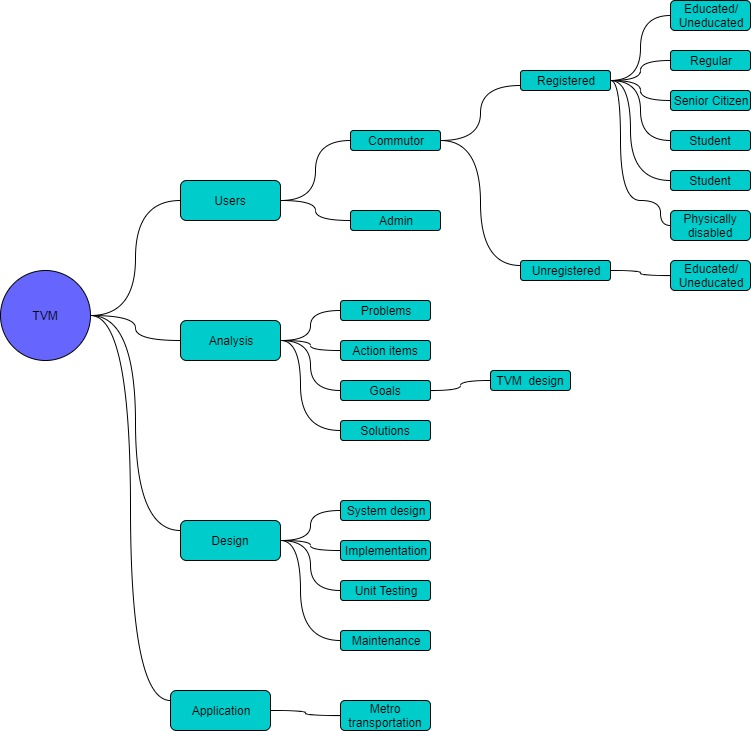
\includegraphics[width=18cm,height=18cm]{Use_Case_Diagrams/MindMap_TVM.jpg}}
	\caption{Mind Map}
	\label{fig: mind_map}
\end{figure}


\subsection{Context of Use Model: User}

\setlength{\tabcolsep}{18pt}
\renewcommand{\arraystretch}{1.5}
\begin{tabular}[H]{ |p{3cm}|p{12cm}| }
	\hline
	\textbf{Factor}  & \textbf{Description}  \\
	\hline
	\textbf{User} &   \\
	\hline
	Role &
	User is the customer/passenger to purchase tickets
	\\
	\hline
	Experience & 
	The experience depends on the how frequent the user is using the TVM, System is designed keeping in mind of a new user without any system knowledge
	\\
	\hline
	Education &
	System is designed assuming that customer can atleast read English. \textbf{constraint:} We wont be able to design a model for who cant read
	\\
	\hline
	Physical Characteristics    &
	The physical TVM should be designed in such a way that even the physically challenged customer with wheel chair should also access the TVM.
	\\
	\hline
	Cognitive Characteristics & 
	The cognitive knowledge of a user should be counted as minimal, the system is designed keeping in mind of new user
	\\
	\hline
	Location & 
	The location of user must be inside Montreal city.
	\\
	\hline
	Age & 
	The system should offer \gls{reduced_fare} according to the user's age.
	\\
	\hline
	Profession & 
	The system should offer reduced fares for students.
	\\
	\hline
	Special Variant Preferences in UI & 
	For special need people with visual impairment system should offer voice messages.
	\\
	\hline
	\textbf{Task} &  \\
	\hline
	Choice in system use &
	Number of tasks in the system should be divided individually, so that the user can choose the options such as purchasing for a single trip, buying a monthly pass etc
	\\
	\hline
	Complexity & 
	Since the users can be with minimal knowledge on the TVM, tasks should be simple and straight forward
	\\
	\hline
	Demands &
	Available tasks should be able to satisfy user requirements with context of use. For example system should not issue more tickets that the number of passengers 
	\\
	\hline 
\end{tabular}


\setlength{\tabcolsep}{18pt}
\renewcommand{\arraystretch}{1.5}
\begin{tabular}[H]{ |p{3cm}|p{12cm}| }
	\hline
	Workflow Controllability & The workflow of each task in TVM machine should be easily controllable by the user. For example user should be able to navigate back to the main menu, user should be able to cancel the ticket selection or transaction etc.\\
	\hline
	Safety & 
	The task payment should be made safer, in such a way that the card payment authentication is kept confidential. Even the user information if stored should be maintained confidential.\\
	\hline
	Criticality & 
	Task criticality should be divided based on the how important the task is and how often it is used/reused.\\
	\hline
	Frequency & 
	The TVM can be used any number of times by any number of users, so the TVM should be able to guide each user based on the current information available with respect to trains or buses.\\
	\hline
	Temporal Characteristics & 
	According to user requests that are dependant to date, the system should validate the request based on current date. \\
	\hline
	\textbf{Environment} & \\
	\hline
	Physical Environment & 
	The TVM will be placed in metro stations, the passengers will be able to buy ticket/passes before there journey in train/bus. The factors like lights on the TVM machine for the visibility, space available to access the TVM, is the place allocated is too noisy should be taken care. \\
	\hline
	Technical Environment & 
	The TVM will be connected to the data server where the user informations can be retrieved, it will be connected to the bank server to authenticate the credit/debit cards. \\
	\hline
	Social Environment & 
	The TVM must support at least two languages including English and French since the official language of Quebec is French. \\
	\hline
\end{tabular}





\subsection{Context of Use Model: Admin}

\setlength{\tabcolsep}{18pt}
\renewcommand{\arraystretch}{1.5}
\begin{tabular}[H]{ |p{3cm}|p{12cm}| }
	\hline
	\textbf{Factor}  & \textbf{Description}  \\
	\hline
	\textbf{Admin} &   \\
	\hline
	Role &
	ADMIN \textbf{constraint:} Due to the data privacy, The admin of TVM real activities were not available
	\\
	\hline
	Experience & 
	The experience depends on the how frequent the admin is using the TVM, System is designed keeping in mind of a new admin without any system knowledge
	\\
	\hline
	Education &
	System is designed assuming that admin can atleast read English \textbf{constraint:} We wont be able to design a model for who cant read
	\\
	\hline
	Physical Characteristics    &
	The physical TVM should be designed in such a way that even the physically challenged admin with wheel chair should also access the TVM
	\\
	\hline
	Cognitive Characteristics & 
	The cognitive knowledge of a admin should be counted as minimal, the system is designed keeping in mind of a new admin
	\\
	\hline
	Location & 
	The location of admin must be inside Montreal city
	\\
	\hline
	Age & 
	Ranging from 25-Retirement age
	\\
	\hline
	Profession & 
	The Profession is Role of the admin
	\\
	\hline
	Special Variant Preferences in UI & 
	For special need people with visual impairment system should offer voice messages
	\\
	\hline
	\textbf{Task} &  \\
	\hline
	Choice in system use &
	Admin should be able to do all administrative activities such changing changing the ticket/monthly pass fares,changing discount offers. Or any User specific actions
	\\
	\hline
	Complexity & 
	Since the admins can be with minimal knowledge on the TVM, tasks should be simple and straight forward
	\\
	\hline
	Demands &
	Should provide the TVM features in such a way, it should be easy for an admin change any relevant activity 
	\\
	\hline 
\end{tabular}


\setlength{\tabcolsep}{18pt}
\renewcommand{\arraystretch}{1.5}
\begin{tabular}[H]{ |p{3cm}|p{12cm}| }
	\hline
	Workflow Controllability & 
	The workflow of each task in TVM machine should be easily controllable by the admin. For example admin should be able to navigate back to the main menu, admin should be able to any discount option, any membership or any user sepefic options\\
	\hline
	Safety & 
	It should be confidential about the admin features. It should be isolated from the normal user login\\
	\hline
	Criticality & 
	Task criticality should be divided based on the how important the task is and how often it is used/reused.\\
	\hline
	Frequency & 
	The TVM can be used any number of times by any number of users, so the TVM should be able to guide each user based on the current information available with respect to trains or buses.\\
	\hline
	Temporal Characteristics & 
	According to admin requests that are dependant to date, the system should validate the request based on current date \\
	\hline
	\textbf{Environment} & \\
	\hline
	Physical Environment & 
	The TVM will be placed in metro stations, the passengers will be able to buy ticket/passes before there journey in train/bus. The factors like lights on the TVM machine for the visibility, space available to access the TVM, is the place allocated is too noisy should be taken care \\
	\hline
	Technical Environment & 
	The TVM will be connected to the data server where the admin informations can be retrieved, it will be connected to the bank server to authenticate the credit/debit cards. \\
	\hline
	Social Environment & 
	The TVM must support at least two languages including English and French since the official language of Quebec is French \\
	\hline
\end{tabular}





%==============================================================
%
%				PROBLEM 3: DOMAIN MODEL
%
%==============================================================

\newpage


\section{Problem 3}
\subsection{Domain Model}
\setlength{\tabcolsep}{18pt}
\renewcommand{\arraystretch}{1.5}
\begin{tabular}[H]{ |p{3cm}|p{12cm}| }
	\hline
	\textbf{Concepts}  & \textbf{Description}  \\
	\hline
	TVM & It is a ticket vending machine to issue ticket or reload rechargeable card for bus and metro
	\\
	\hline
	User & Someone who uses TVM as a commuter, an administrator or a negative user as a crook
	\\
	\hline
	Administrator & Someone who has privilege to manage ticket specification
	\\
	\hline
	Crook & A negative user how tries to misuse the TVM like a hacker who is trying to steal bank car information
	\\
	\hline
	Commuter & Someone who comes to TVM and wants to buy ticket or check different fares to travel
	\\
	\hline
	Registered Commuter & Someone who has registered his/her information in the system and uses their Rechargeable Card to buy ticket
	\\
	\hline
	Unregistered Commuter & Someone who has not registered his/her information in the system and uses the system anonymously and buy Non-Rechargeable Ticket
	\\
	\hline
	Student & Someone who has the proof of being a student and is eligible to use reduced fare
	\\
	\hline
	Regular & Someone who has registered in the system and use Rechargeable Card, but pay \gls{regular_fare}
	\\
	\hline
	Senior Citizen & Someone who is 65 years old or over and is eligible to use reduced fare
	\\
	\hline
	Language & The display language of User Interface that can be either English or French
	\\
	\hline
	Printer & Printer is the device that prints the receipt or provides the non-rechargeable ticket
	\\
	\hline 
	Receipt & It has the confirmation of the transaction and this is the superclass of different kinds of receipt
	\\
	\hline
\end{tabular}
	
\setlength{\tabcolsep}{18pt}
\renewcommand{\arraystretch}{1.5}
\begin{tabular}[H]{ |p{3cm}|p{12cm}| }
	\hline
	Paper Receipt & It is a subclass of receipt which is printed on paper
	\\
	\hline
	Email & It is subclass of receipt electronically delivered to the user
	\\
	\hline
	Ticket & It is either a rechargeable or non-rechargeable ticket which users pay for to use metro or bus
	\\
	\hline
	Ticket Type & It describes number of trips or the duration (e.g. monthly ticket) of the ticket
	\\
	\hline
	Non-Rechargeable Ticket & It is a temporary ticket for limited use printed on the paper by printer
	\\
	\hline
	Rechargable Card & A card which has an expiry date and can be recharged and used multiple times before the expiration date
	\\
	\hline
	Fare & It includes the price of different plans to buy the ticket
	\\
	\hline
	Regular & It is regular price of a specific plan
	\\
	\hline
	Reduced & It is reduced price of a specific plan for special customers such as students or people with certain ages
	\\
	\hline
	Payment & It is superclass for different modes of payment
	\\
	\hline
	Bank Card & It is a payment method that uses bank card to pay for the ticket fare
	\\
	\hline
	Cash & It is a payment method that uses cash to pay for the ticket fare
	\\
	\hline
	Transaction & It debits customer bank card  
	\\
	\hline
	Payment Authentication & It takes the details of the user’s bank card and verify the payment with the bank server
	\\
	\hline
	Bank Server & It confirms user’s bank card information
	\\
	\hline
\end{tabular}
\\ 


\newpage

\begin{figure}[!htb]
	\centering
	\fbox{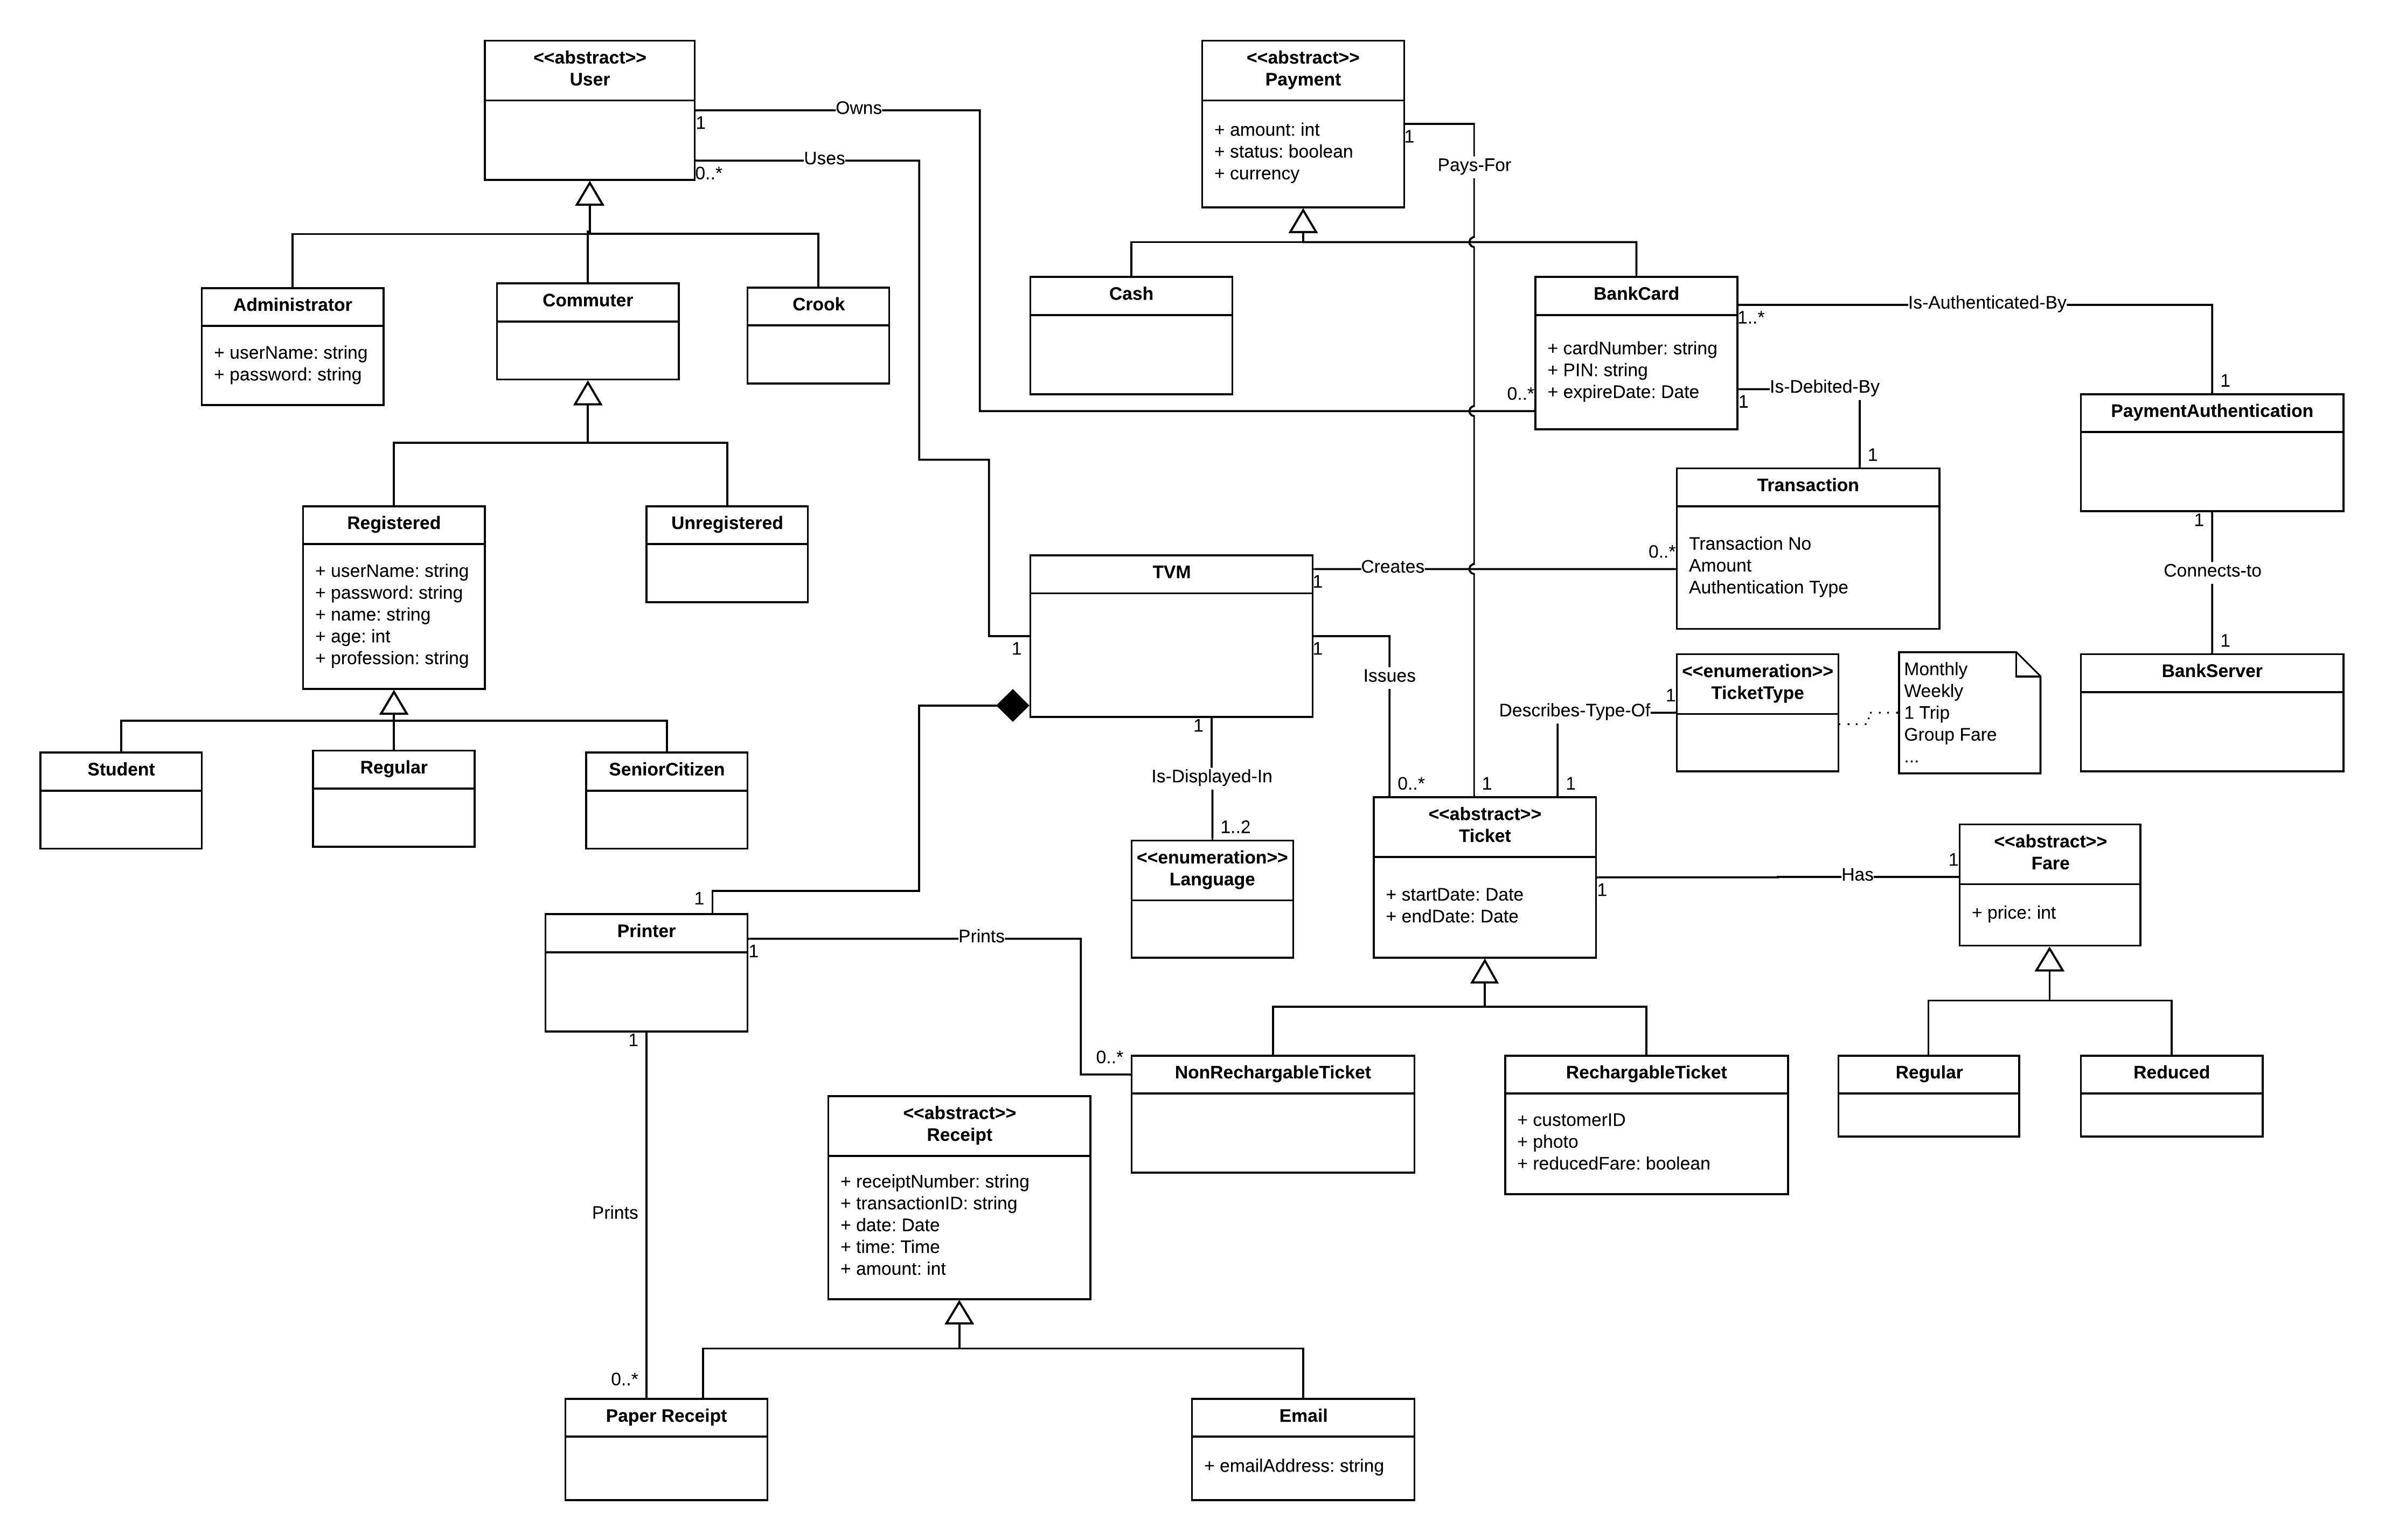
\includegraphics[width=18cm,height=20cm]{domain_model.jpeg}}
	\caption{\label{fig:Domain Model} Domain Model}	
\end{figure}


%==============================================================
%
%				PROBLEM 4: USE CASE MODEL
%
%==============================================================

\newpage

\FloatBarrier
\section{Problem 4}

\FloatBarrier
\subsection{Use Case Model}
\begin{figure}[!htb]
	\fbox{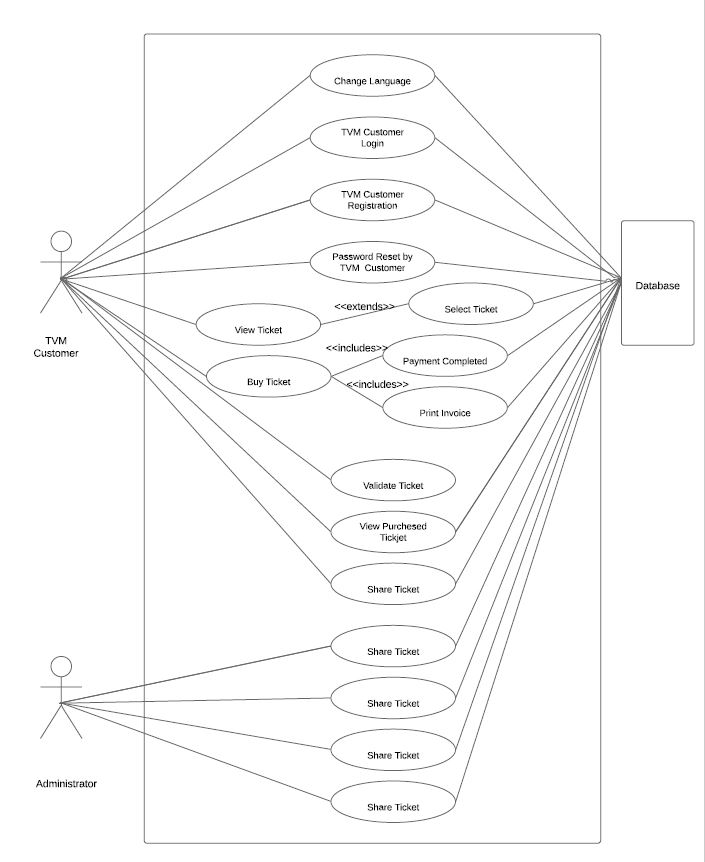
\includegraphics[width=18cm, height=18cm]{Use_Case_Diagrams/UseCaseModel.JPG}}
	\caption{\label{fig:uc_use_case_model} Use Case Model}	
\end{figure}


\FloatBarrier
\subsection{Use Case: Change Language}
 
\begin{tabular}{ | c | p{2cm} | p{7cm} |}
	
	\hline
	\textbf{Number} & \multicolumn{2}{c|}{1}  \\
	\hline
	\textbf{Name} & \multicolumn{2}{c|}{Change Language}  \\
	\hline
	\textbf{Summary} & \multicolumn{2}{c|}{User wants to change to desired language }  \\
	\hline
	\textbf{Priority} & \multicolumn{2}{c|}{4}  \\
	\hline
	\textbf{Preconditions} & \multicolumn{2}{c|}{N/A}  \\
	\hline
	\textbf{Postconditions} & \multicolumn{2}{c|}{User is able to change to desired language}  \\
	\hline
	\textbf{Primary Actor(s)} & \multicolumn{2}{c|}{TVM Customer}  \\
	\hline
	\textbf{Secondary Actors(s)} & \multicolumn{2}{c|}{TVM and Administrator}  \\
	\hline
	\textbf{Trigger} & \multicolumn{2}{c|}{User has chosen to change language}  \\
	\hline
	\textbf{Main Success Scenarios} & \textbf{Step} & \textbf{Action} \\
	\hline
	  & 1 & User can select the desired language \\ 
	\hline
	  &  2  & The application is displayed in desired language \\
	\hline
	\textbf{Extensions} & \multicolumn{2}{c|}{N/A}  \\
	\hline
	\textbf{Open Issues} &  1  & Language available to be decided by the customer \\
	\hline
\end{tabular}



\FloatBarrier

\subsection{Use Case: View Ticket Plans}
Commuters use Ticket vending machine to view ticket plans. Commuter is the primary actor that initiate the use case by choosing to view ticket plans.Secondary actor includes Data Store that supports and responds to the requests. The result for a normal use case scenario is that the customer has viewed different ticket plans. Figure~\ref{fig:uc_view_ticket_plans} explain this use case. \\

\begin{tabular}{ | c | p{2cm} | p{7cm} |}
	
	\hline
	\textbf{Number} & \multicolumn{2}{c|}{2}  \\
	\hline
	\textbf{Name} & \multicolumn{2}{c|}{View Ticket Plans}  \\
	\hline
	\textbf{Summary} & \multicolumn{2}{c|}{User has viewed different ticket plans}  \\
	\hline
	\textbf{Priority} & \multicolumn{2}{c|}{1}  \\
	\hline
	\textbf{Preconditions} & \multicolumn{2}{c|}{N/A}  \\
	\hline
	\textbf{Postconditions} & \multicolumn{2}{c|}{User has viewed different ticket plans}  \\
	\hline
	\textbf{Primary Actor(s)} & \multicolumn{2}{c|}{TVM Customer}  \\
	\hline
	\textbf{Secondary Actors(s)} & \multicolumn{2}{c|}{Data Store}  \\
	\hline
	\textbf{Trigger} & \multicolumn{2}{c|}{User has chosen to view ticket plans}  \\
	\hline
	\textbf{Main Success Scenarios} & \textbf{Step} & \textbf{Action} \\
	\hline
	& 1 & User selects the language \\ 
	\hline
	&  2  & System asks the ticket type \\
	\hline
	&  3  & User selects the ticket type \\
	\hline
	&  2  & System displays ticket plans \\
	\hline
	\textbf{Extensions} & \multicolumn{2}{c|}{N/A}  \\
	\hline
	\textbf{Open Issues} &    & NA \\
	\hline
	
\end{tabular}

\begin{figure}[!htb]
	\fbox{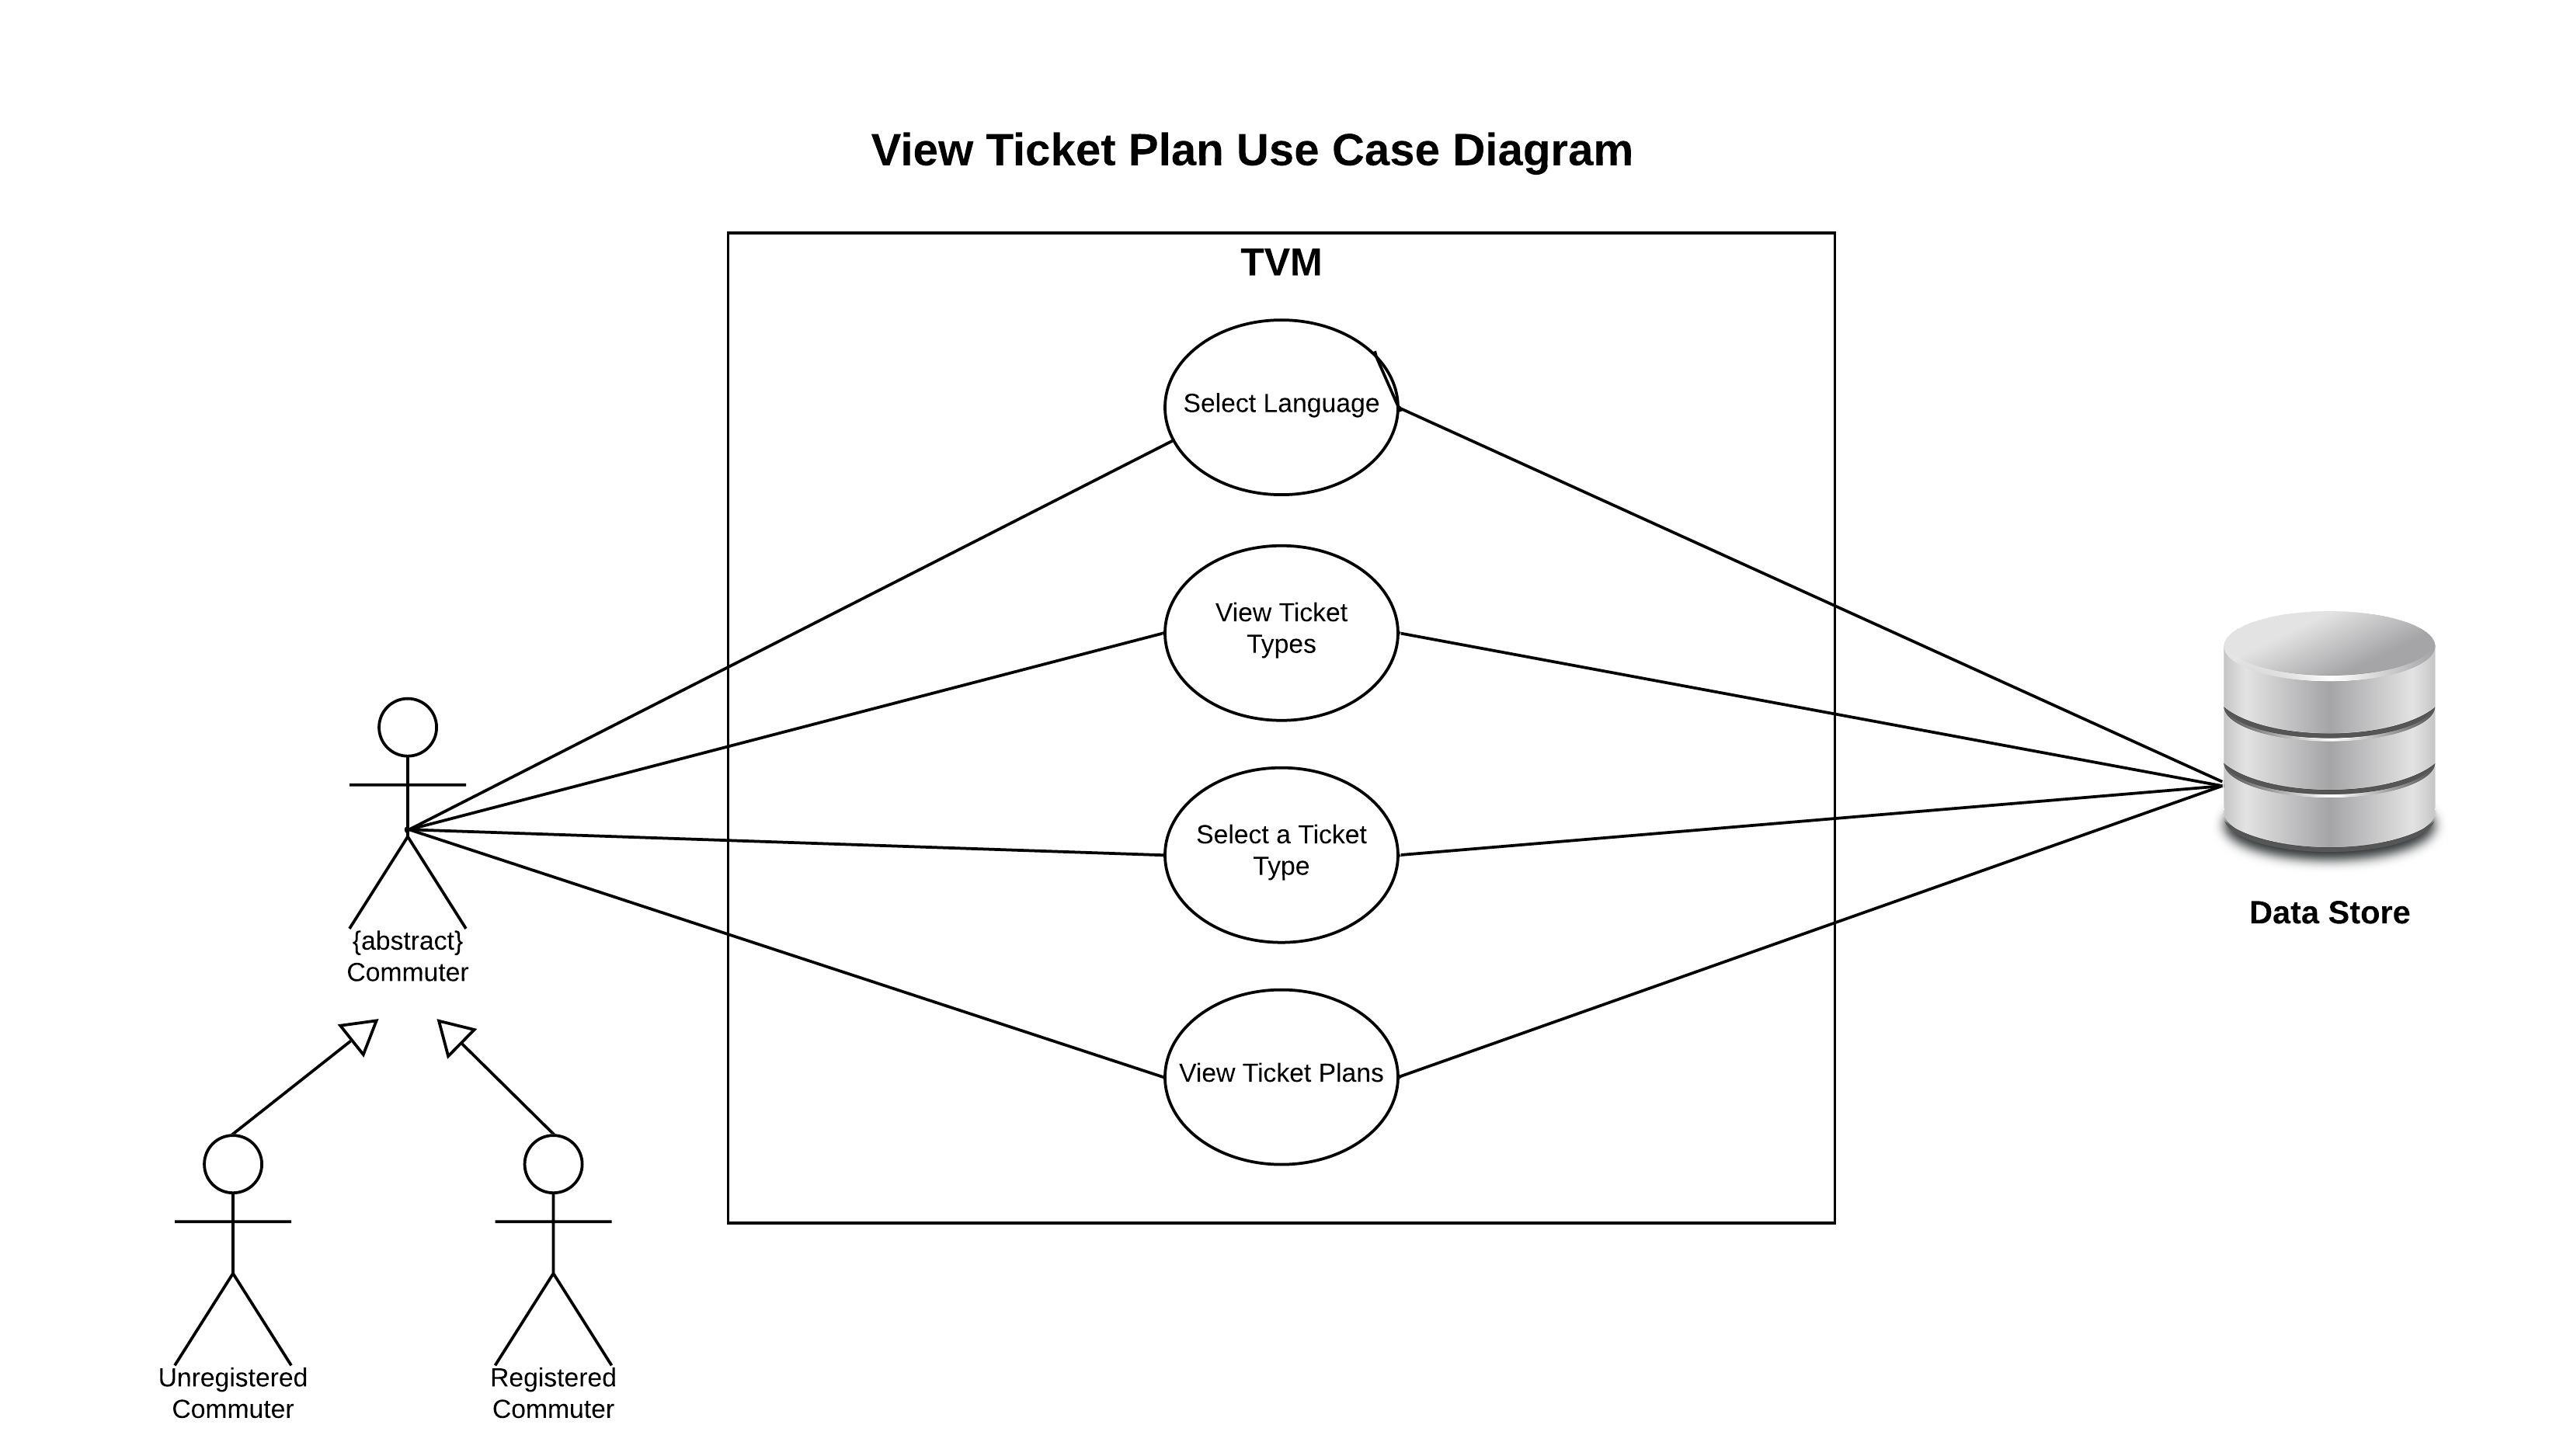
\includegraphics[width=18cm, height=16cm]{Use_Case_Diagrams/ViewTicketPlan.jpeg}}
	\caption{\label{fig:uc_view_ticket_plans}Use Case: View Ticket Plans}	
\end{figure}





\FloatBarrier
\subsection{Use Case: Buy Tickets}
Commuters use Ticket vending machine to buy tickets. Commuter is the primary actor that initiate the use case by choosing to buy a ticket. Secondary actors include Payment Authentication and Data Store that support and respond to the requests. The result for a normal use case scenario is that the customer has received the ticket and the receipt. Figure~\ref{fig:uc_buy_ticket} and~\ref{fig:act_buy_ticket} and~\ref{fig:seq_buy_ticket} explain this use case. \\ 

\begin{tabular}{ | c | p{2cm} | p{7cm} |}
	
	\hline
	\textbf{Number} & \multicolumn{2}{c|}{3}  \\
	\hline
	\textbf{Name} & \multicolumn{2}{c|}{Buy Ticket}  \\
	\hline
	\textbf{Summary} & \multicolumn{2}{c|}{Customer buy a ticket using TVM}  \\
	\hline
	\textbf{Priority} & \multicolumn{2}{c|}{1}  \\
	\hline
	\textbf{Preconditions} & \multicolumn{2}{c|}{Customer has access to a valid payment method}  \\
	\hline
	\textbf{Postconditions} & \multicolumn{2}{c|}{Customer has received the ticket and the receipt}  \\
	\hline
	\textbf{Primary Actor(s)} & \multicolumn{2}{c|}{TVM Customer}  \\
	\hline
	\textbf{Secondary Actors(s)} & \multicolumn{2}{c|}{Payment Authentication, Bank Server, Data Store}  \\
	\hline
	\textbf{Trigger} & \multicolumn{2}{c|}{Customer has chosen to buy a ticket}  \\
	\hline
	\textbf{Main Success Scenarios} & \textbf{Step} & \textbf{Action} \\
	\hline
	& 1 & Customer selects the language \\ 
	\hline
	&  2  & System displays ticket plans \\
	\hline
	&  3  & Customer chooses a ticket plan \\
	\hline
	&  4  & System asks for payment method \\
	\hline
	&  5  & Customer selects a payment method \\
	\hline
	&  6  & Customer makes a payment \\
	\hline
	&  7  & System asks for type of receipt \\
	\hline
	&  8  & Customer selects the type of receipt \\
	\hline
	&  9  & System prints receipt and ticket \\
	\hline
	&  10  & Customer removes receipt and ticket \\
	\hline
	&  11  & System displays welcome message \\
	\hline
	\textbf{Extensions} & \textbf{Step} & \textbf{Branching Action} \\
	\hline
	&  6a  & The payment is not successful \\
	\hline
	&  6b  & System displays message that payment is not successful \\
	\hline
	&  6c  & System exits and displays welcome message \\
	\hline
	\textbf{Open Issues} &    & NA \\
	\hline
	
\end{tabular}

\newpage

\begin{figure}[!htb]
	\centering
	\fbox{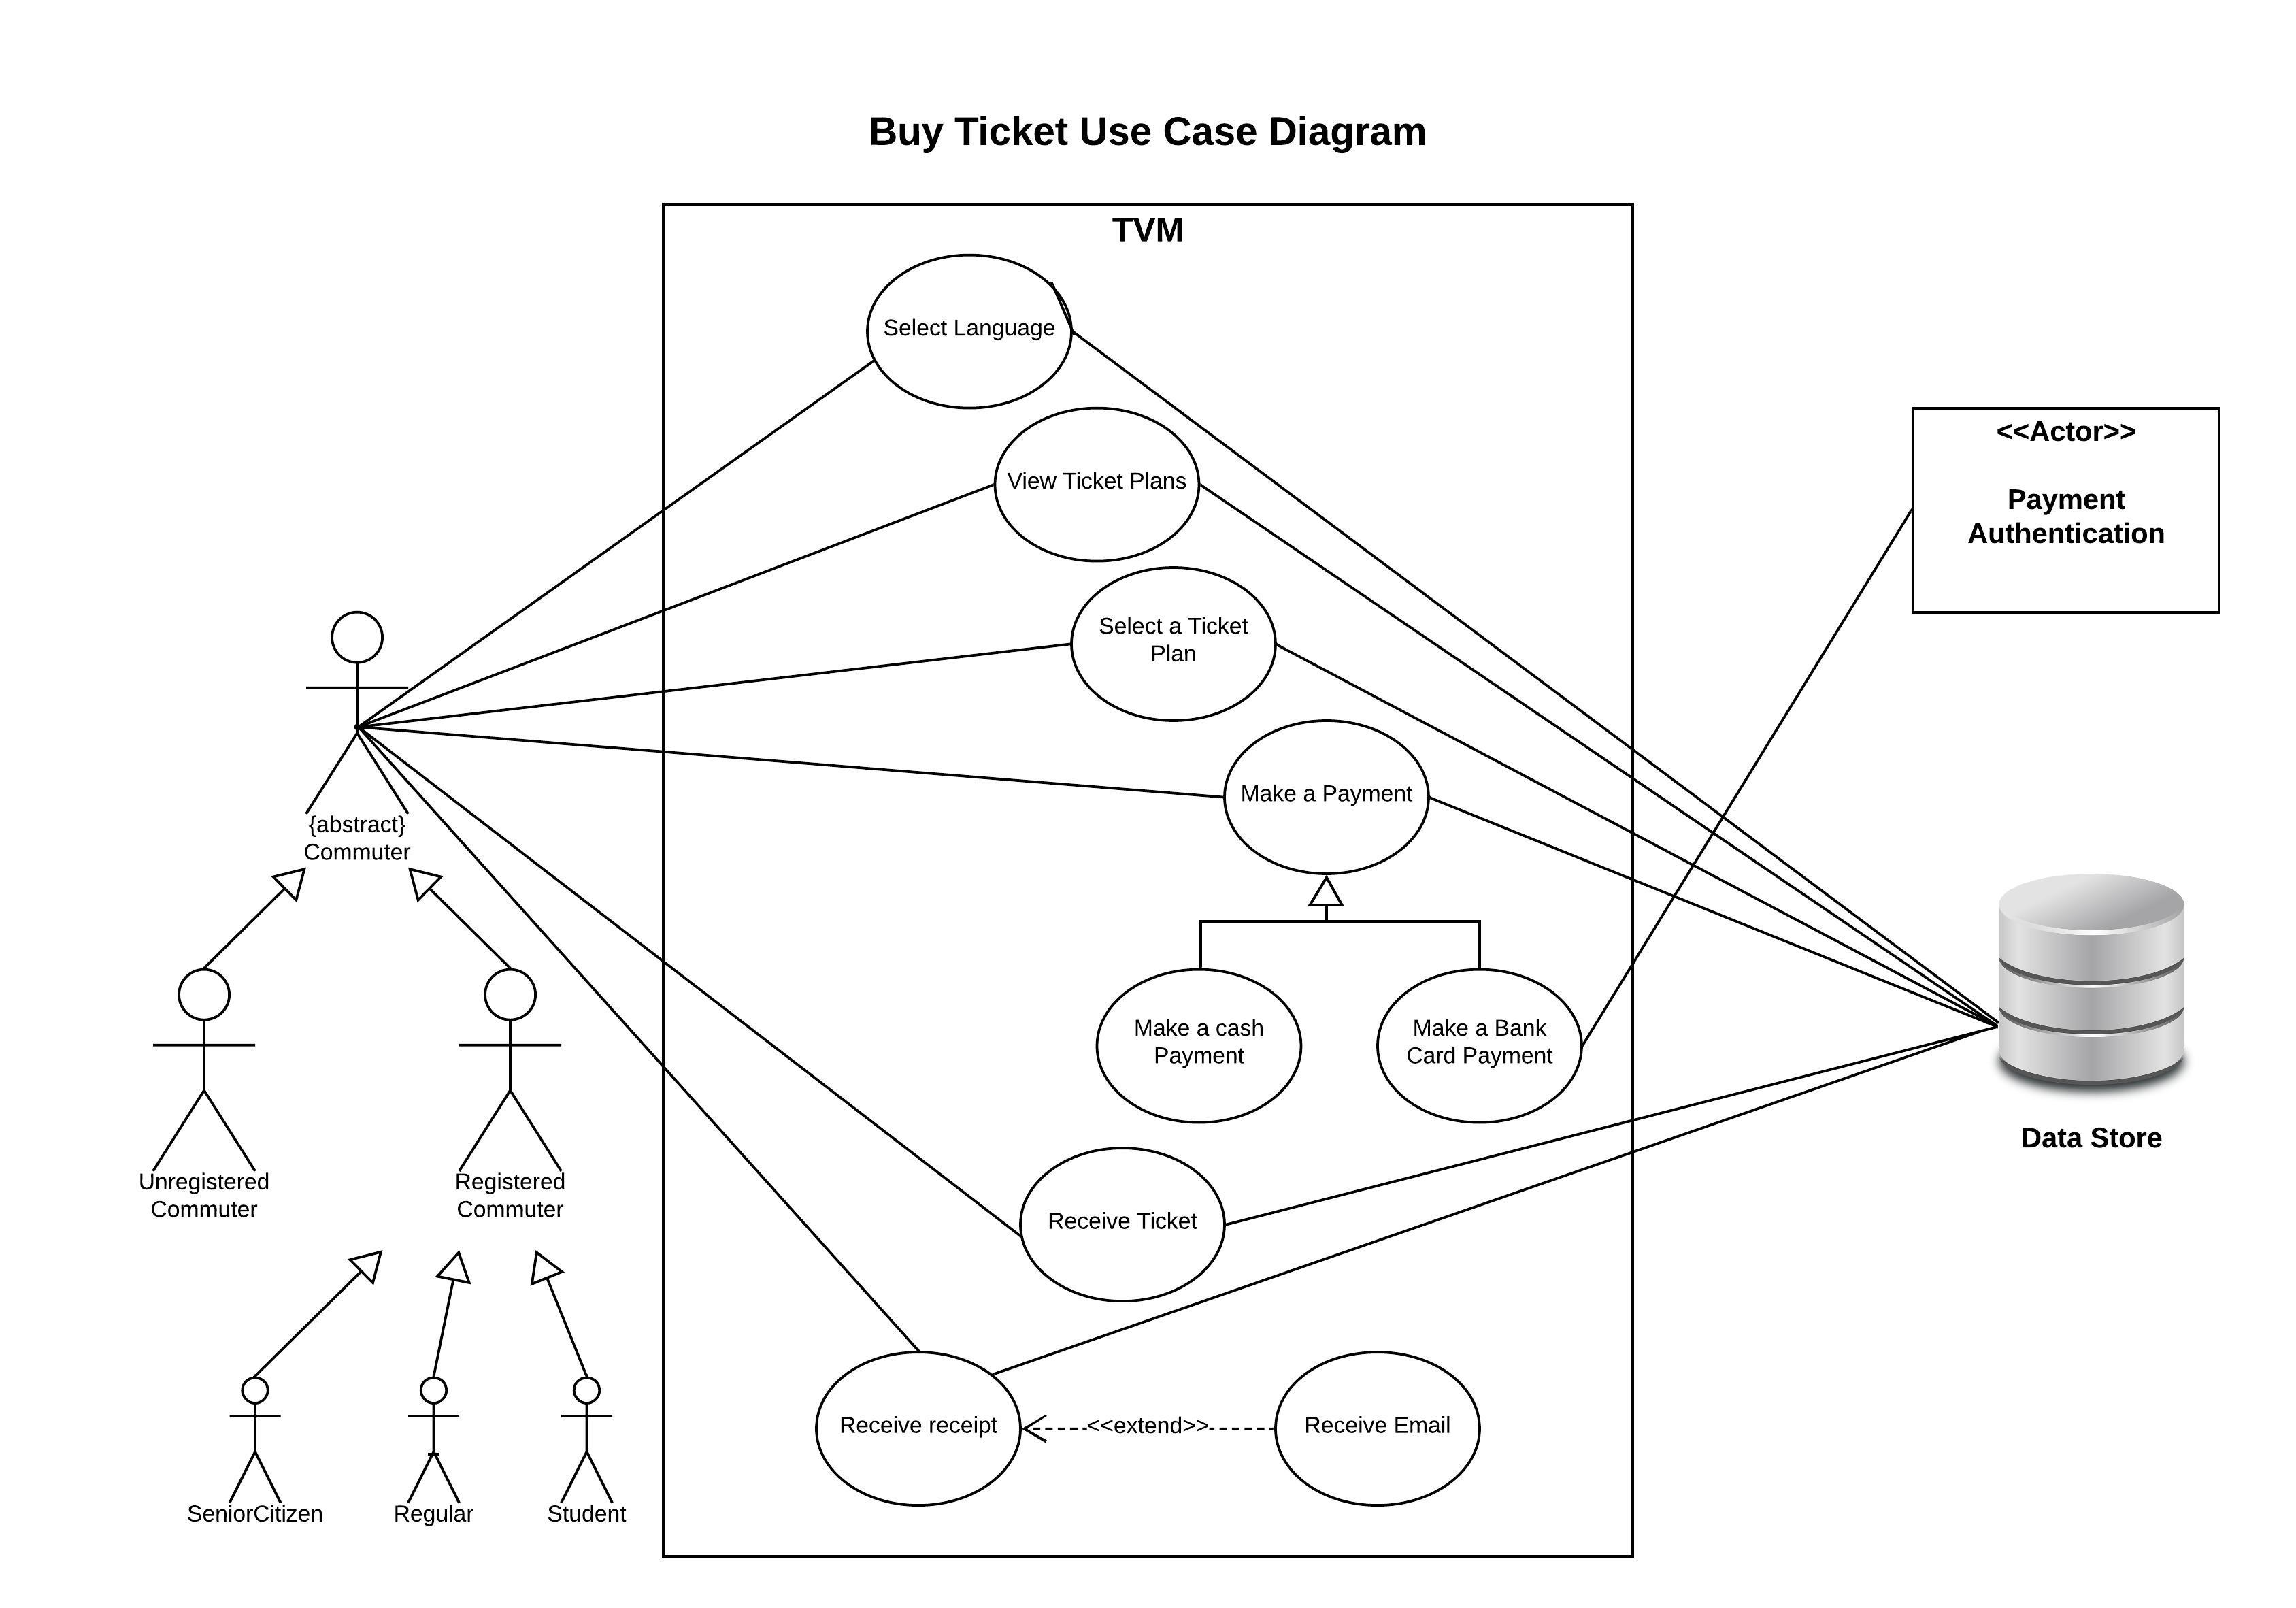
\includegraphics[width=18cm, height=16cm]{Use_Case_Diagrams/BuyTicket.jpeg}}
	\caption{\label{fig:uc_buy_ticket}Use Case: Buy Ticket}	
\end{figure}

\newpage

\begin{figure}[!htbp]
	\centering
	\fbox{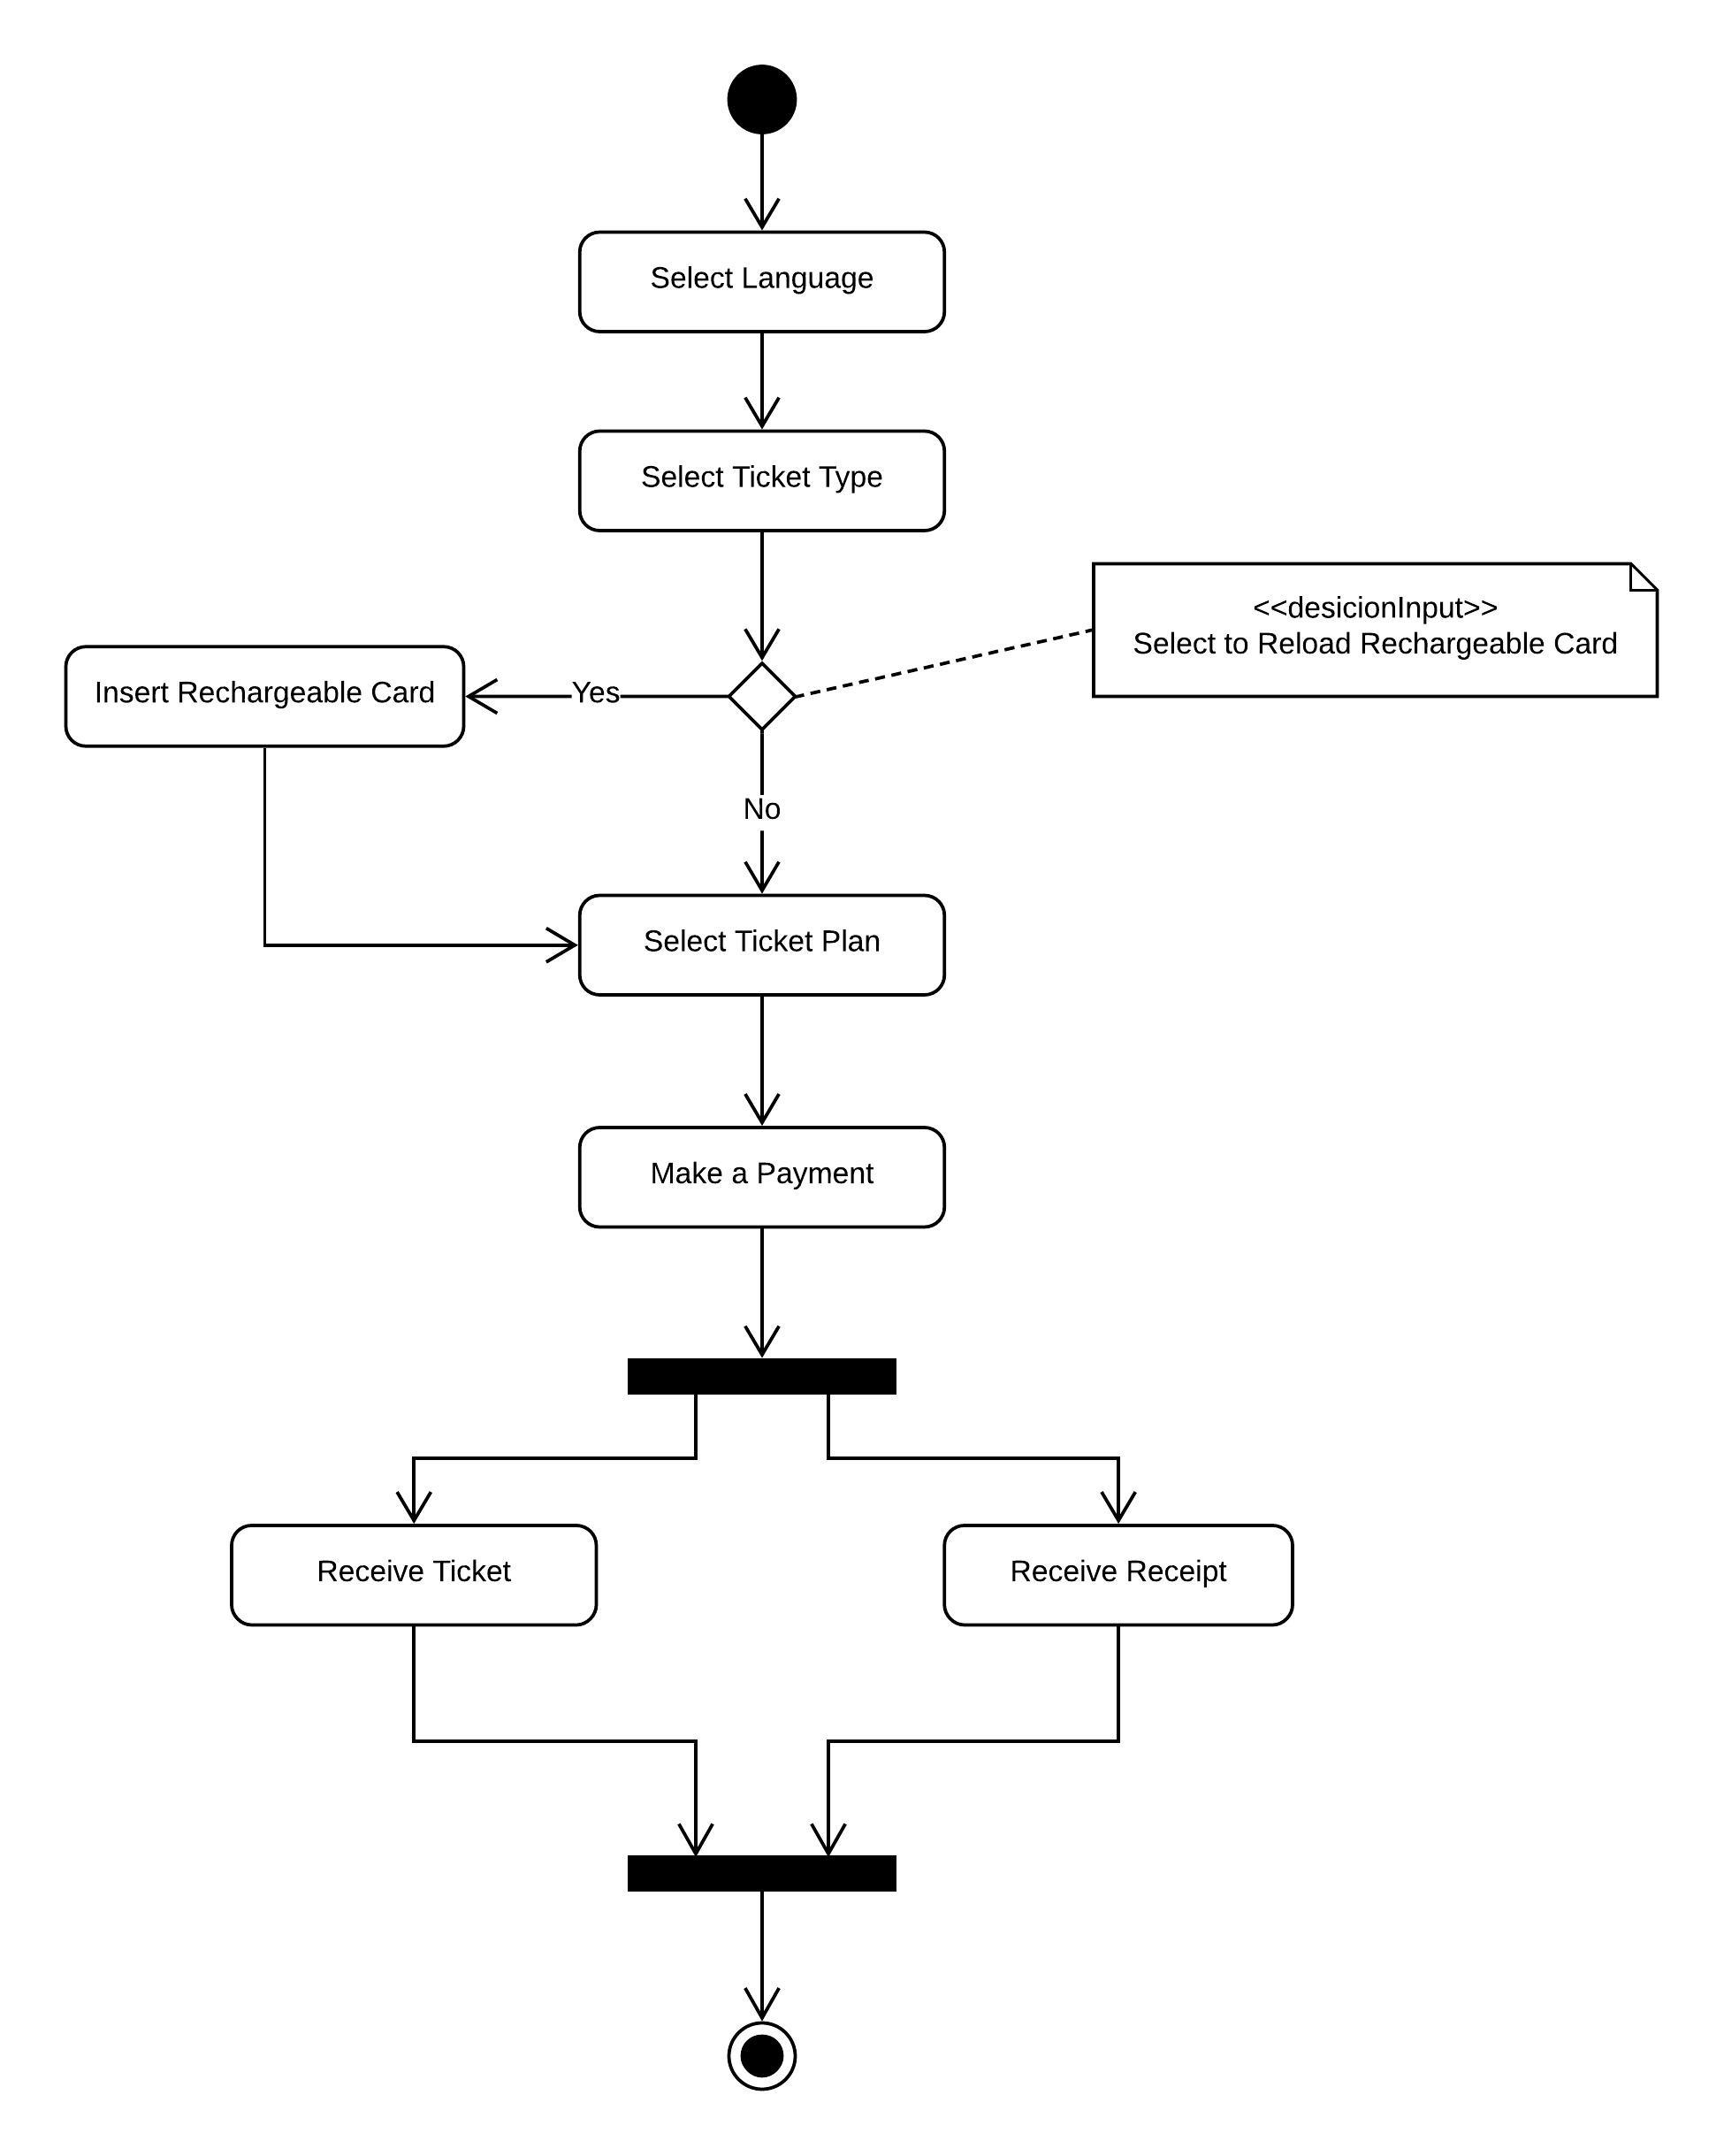
\includegraphics[width=0.9\textwidth]{Use_Case_Diagrams/BuyTicket_AD.jpeg}}
	\caption{\label{fig:act_buy_ticket} Activity Diagram: Buy Ticket}	
\end{figure}

\newpage 

\begin{figure}[!htbp]
	\centering
	\fbox{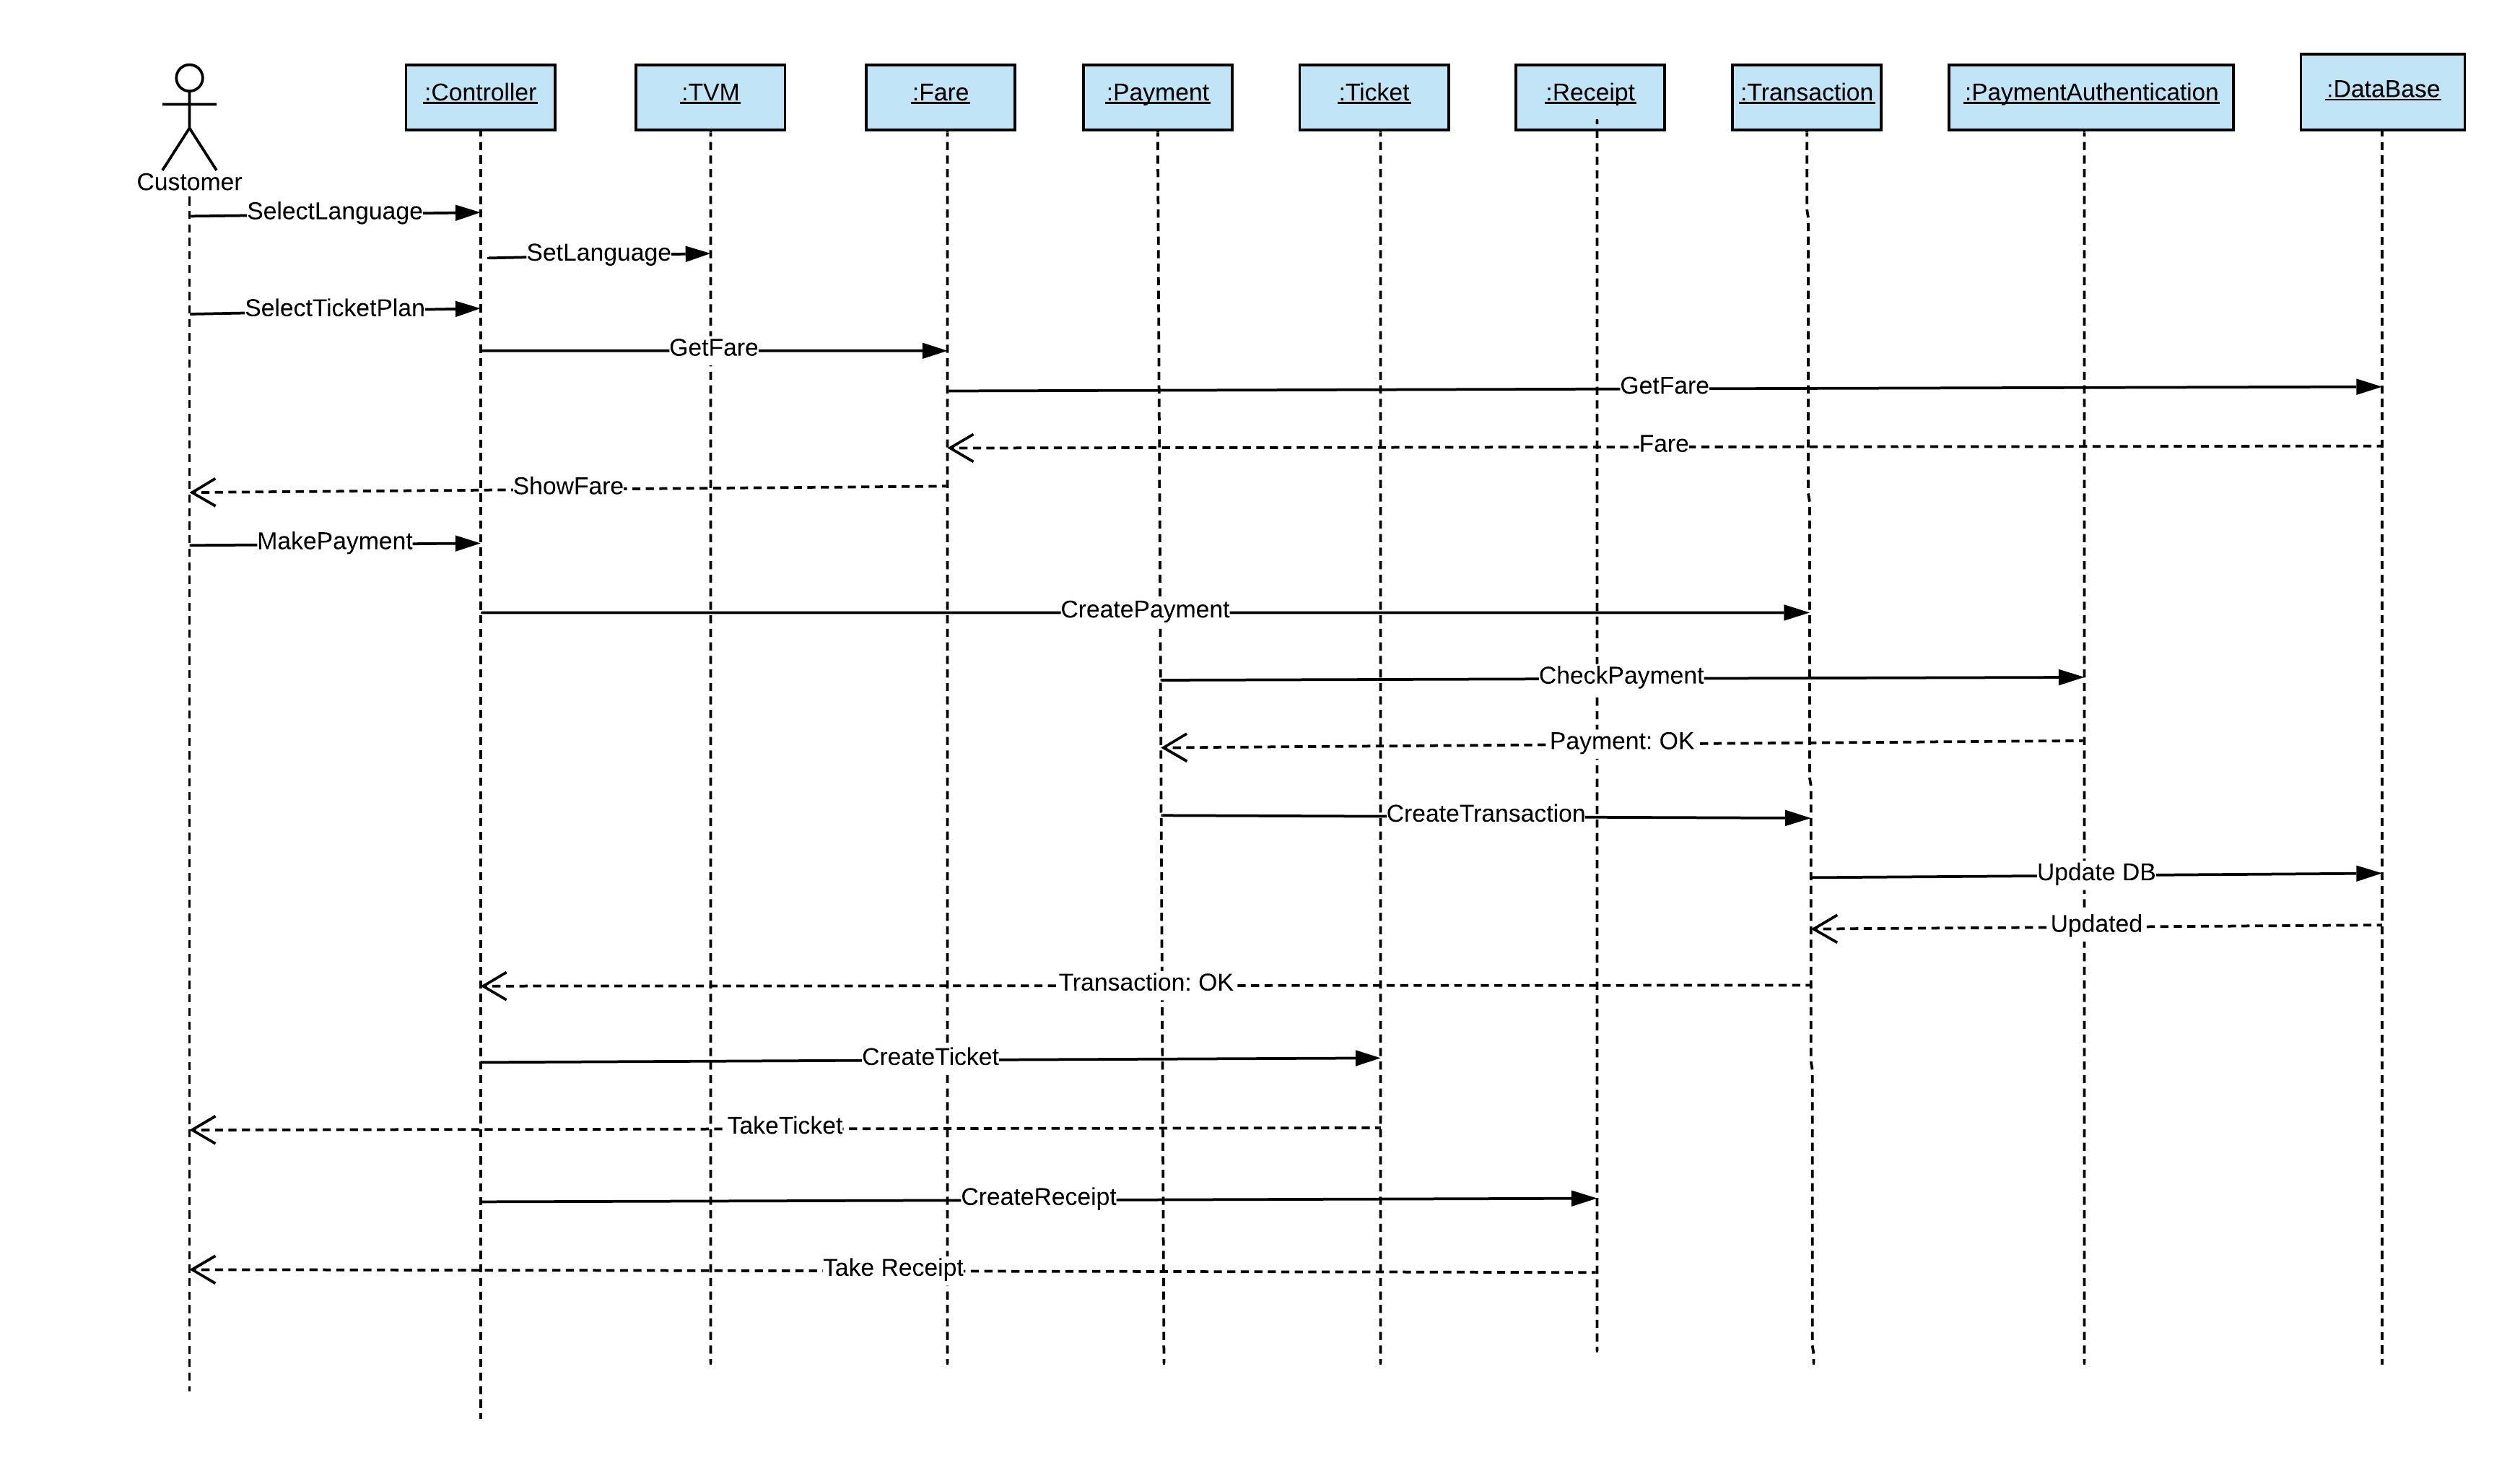
\includegraphics[width=18cm, height=16cm]{Use_Case_Diagrams/BuyTicket_seq.jpeg}}
	\caption{\label{fig:seq_buy_ticket} Sequence Diagram: Buy Ticket}	
\end{figure}





\FloatBarrier
\subsection{Use Case: Make a payment}
Commuters use Ticket vending machine to make payments. Commuter is the primary actor that initiate the use case by choosing ticket plan.Secondary actor includes Data Store that supports and responds to the requests. The result for a normal use case scenario is that the customer has paid for the ticket plan and got the confirmation of payment successfull or not. Figure~\ref{fig:uc_make_payment} explain this use case.

\begin{tabular}{ | c | p{2cm} | p{7cm} |}
	
	\hline
	\textbf{Number} & \multicolumn{2}{c|}{4}  \\
	\hline
	\textbf{Name} & \multicolumn{2}{c|}{Make a Credit Card Payment, Make a cash Payment}  \\
	\hline
	\textbf{Summary} & \multicolumn{2}{c|}{Customer make payment by card or cash using TVM}  \\
	\hline
	\textbf{Priority} & \multicolumn{2}{c|}{1}  \\
	\hline
	\textbf{Preconditions} & \multicolumn{2}{c|}{User has a valid credit card, valid currency}  \\
	\hline
	\textbf{Postconditions} & \multicolumn{2}{c|}{Transaction successful, user should get the ticket.}  \\
	\hline
	\textbf{Primary Actor(s)} & \multicolumn{2}{c|}{TVM Customer / Bank Card Reader / Cash Receiver.}  \\
	\hline
	\textbf{Secondary Actors(s)} & \multicolumn{2}{c|}{Payment Gateway.}  \\
	\hline
	\textbf{Trigger} & \multicolumn{2}{c|}{User has chosen to buy a metro ticket}  \\
	\hline
	\textbf{Main Success Scenarios} & \textbf{Step} & \textbf{Action} \\
	\hline
	& 1 & System displays ticket types \\ 
	\hline
	&  2  & User chooses the type of ticket \\
	\hline
	&  3  & System asks for payment method \\
	\hline
	&  4  & User select pay by cash or card \\
	\hline
	&  5  & System asks user to insert his card or cash (to cash receiver). \\
	\hline
	&  6  & User insert his cash or card. \\
	\hline
	&  7  & System asks user to enter the PIN (in case of card payment) \\
	\hline
	&  8  & User enter the PIN \\
	\hline
	&  9  & System connects to the payment gateway and authentication the user details. \\
	\hline
	&  10  & System create a transaction and records the transaction. \\
	\hline
	&  11  & System asks how user wants to receive the receipt \\
	\hline
	&  12  & User select paper receipt \\
	\hline
	
\end{tabular}


\begin{tabular}{ | c | p{2cm} | p{7cm} |}
	\hline
	&  13  & System prints and dispenses receipt and ticket \\
	\hline
	&  14  & User takes out receipt and ticket. \\
	\hline
	&  15  & System displays a message to remove the credit card \\
	\hline
	&  16  & User removes card \\
	\hline
	&  17  & System displays welcome message. \\
	\hline
	
	\textbf{Extensions} & \textbf{Step} & \textbf{Branching Action} \\
	\hline
	&  6a  & User insert card into card reader. \\
	\hline
	&  6b  & User insert cash into the cash receiver. \\
	\hline
	&  7a  & No pin asked in case of cash payment. \\
	\hline
	&  9a  & System authenticated the cash denominations in case of cash payment. \\
	\hline
	&  11a  & If payment is not successful user will not receive the print receipt message. \\
	\hline
	&  15a  & No message displayed in case of cash payment. \\
	\hline
	\textbf{Open Issues} &    & NA \\
	\hline
	
\end{tabular}


\begin{figure}[!htb]
	\fbox{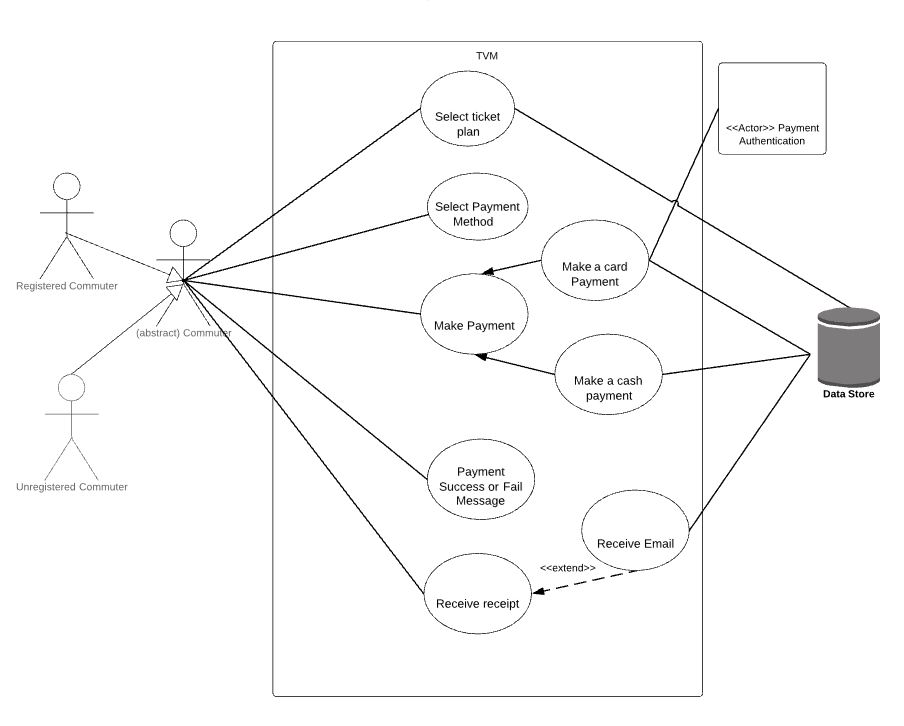
\includegraphics[width=1\textwidth]{Use_Case_Diagrams/MakePayment.JPG}}
	\caption{\label{fig:uc_make_payment}Use Case: Make Payment}	
\end{figure}


\FloatBarrier
\subsection{Use Case: Reload Rechargable Card}
Commuters use Ticket vending machine to recharge their rechargeable card. Commuter is the primary actor that initiate the use case by inserting his/her card. Secondary actors include Payment Authentication and Data Store that support and respond to the requests. The result for a normal use case scenario is that the customer has recharged his /her card and received the receipt. Figure~\ref{fig:uc_reload_rechargable_card} and~\ref{fig:act_reload_rechargable_card} explain this use case. \\

\begin{tabular}{ | c | p{2cm} | p{7cm} |}
	
	\hline
	\textbf{Number} & \multicolumn{2}{c|}{5}  \\
	\hline
	\textbf{Name} & \multicolumn{2}{c|}{Reload Rechargeable Card}  \\
	\hline
	\textbf{Summary} & \multicolumn{2}{c|}{Customer reloads the rechargeable card using TVM}  \\
	\hline
	\textbf{Priority} & \multicolumn{2}{c|}{1}  \\
	\hline
	\textbf{Preconditions} & \multicolumn{2}{c|}{User has a Rechargeable card}  \\
	\hline
	\textbf{Postconditions} & \multicolumn{2}{c|}{User has recharged the card and received a receipt}  \\
	\hline
	\textbf{Primary Actor(s)} & \multicolumn{2}{c|}{TVM Customer}  \\
	\hline
	\textbf{Secondary Actors(s)} & \multicolumn{2}{c|}{Data Store}  \\
	\hline
	\textbf{Trigger} & \multicolumn{2}{c|}{User has chosen to reload the card}  \\
	\hline
	\textbf{Main Success Scenarios} & \textbf{Step} & \textbf{Action} \\
	\hline
	& 1 & User inserts the rechargeable card in the machine \\ 
	\hline
	&  2  & User selects the language \\
	\hline
	&  3  & User select the option to recharge the card \\
	\hline
	&  4  & System displays different recharge plans \\
	\hline
	&  5  & User chooses the recharge plan \\
	\hline
	&  6  & System asks for the payment method \\
	\hline
	&  7  & User choses the way of payment \\
	\hline
	&  8  & User done with the payment \\
	\hline
	&  9  & System displays the message to retrieve the rechargeable card \\
	\hline
	&  10  & User removes the card. \\
	\hline
	&  11  & System asks the user if he wants to print receipt \\
	\hline
	&  12  & User select the option from Yes or No \\
	\hline
	&  13  & System prints and dispenses receipt \\
	\hline
	&  14  & System displays welcome message \\
	\hline
	
	\textbf{Extensions} & \textbf{Step} & \textbf{Branching Action} \\
	\hline
	\textbf{Open Issues} &    & NA \\
	\hline
	
\end{tabular}


\begin{figure}[!htbp]
	\fbox{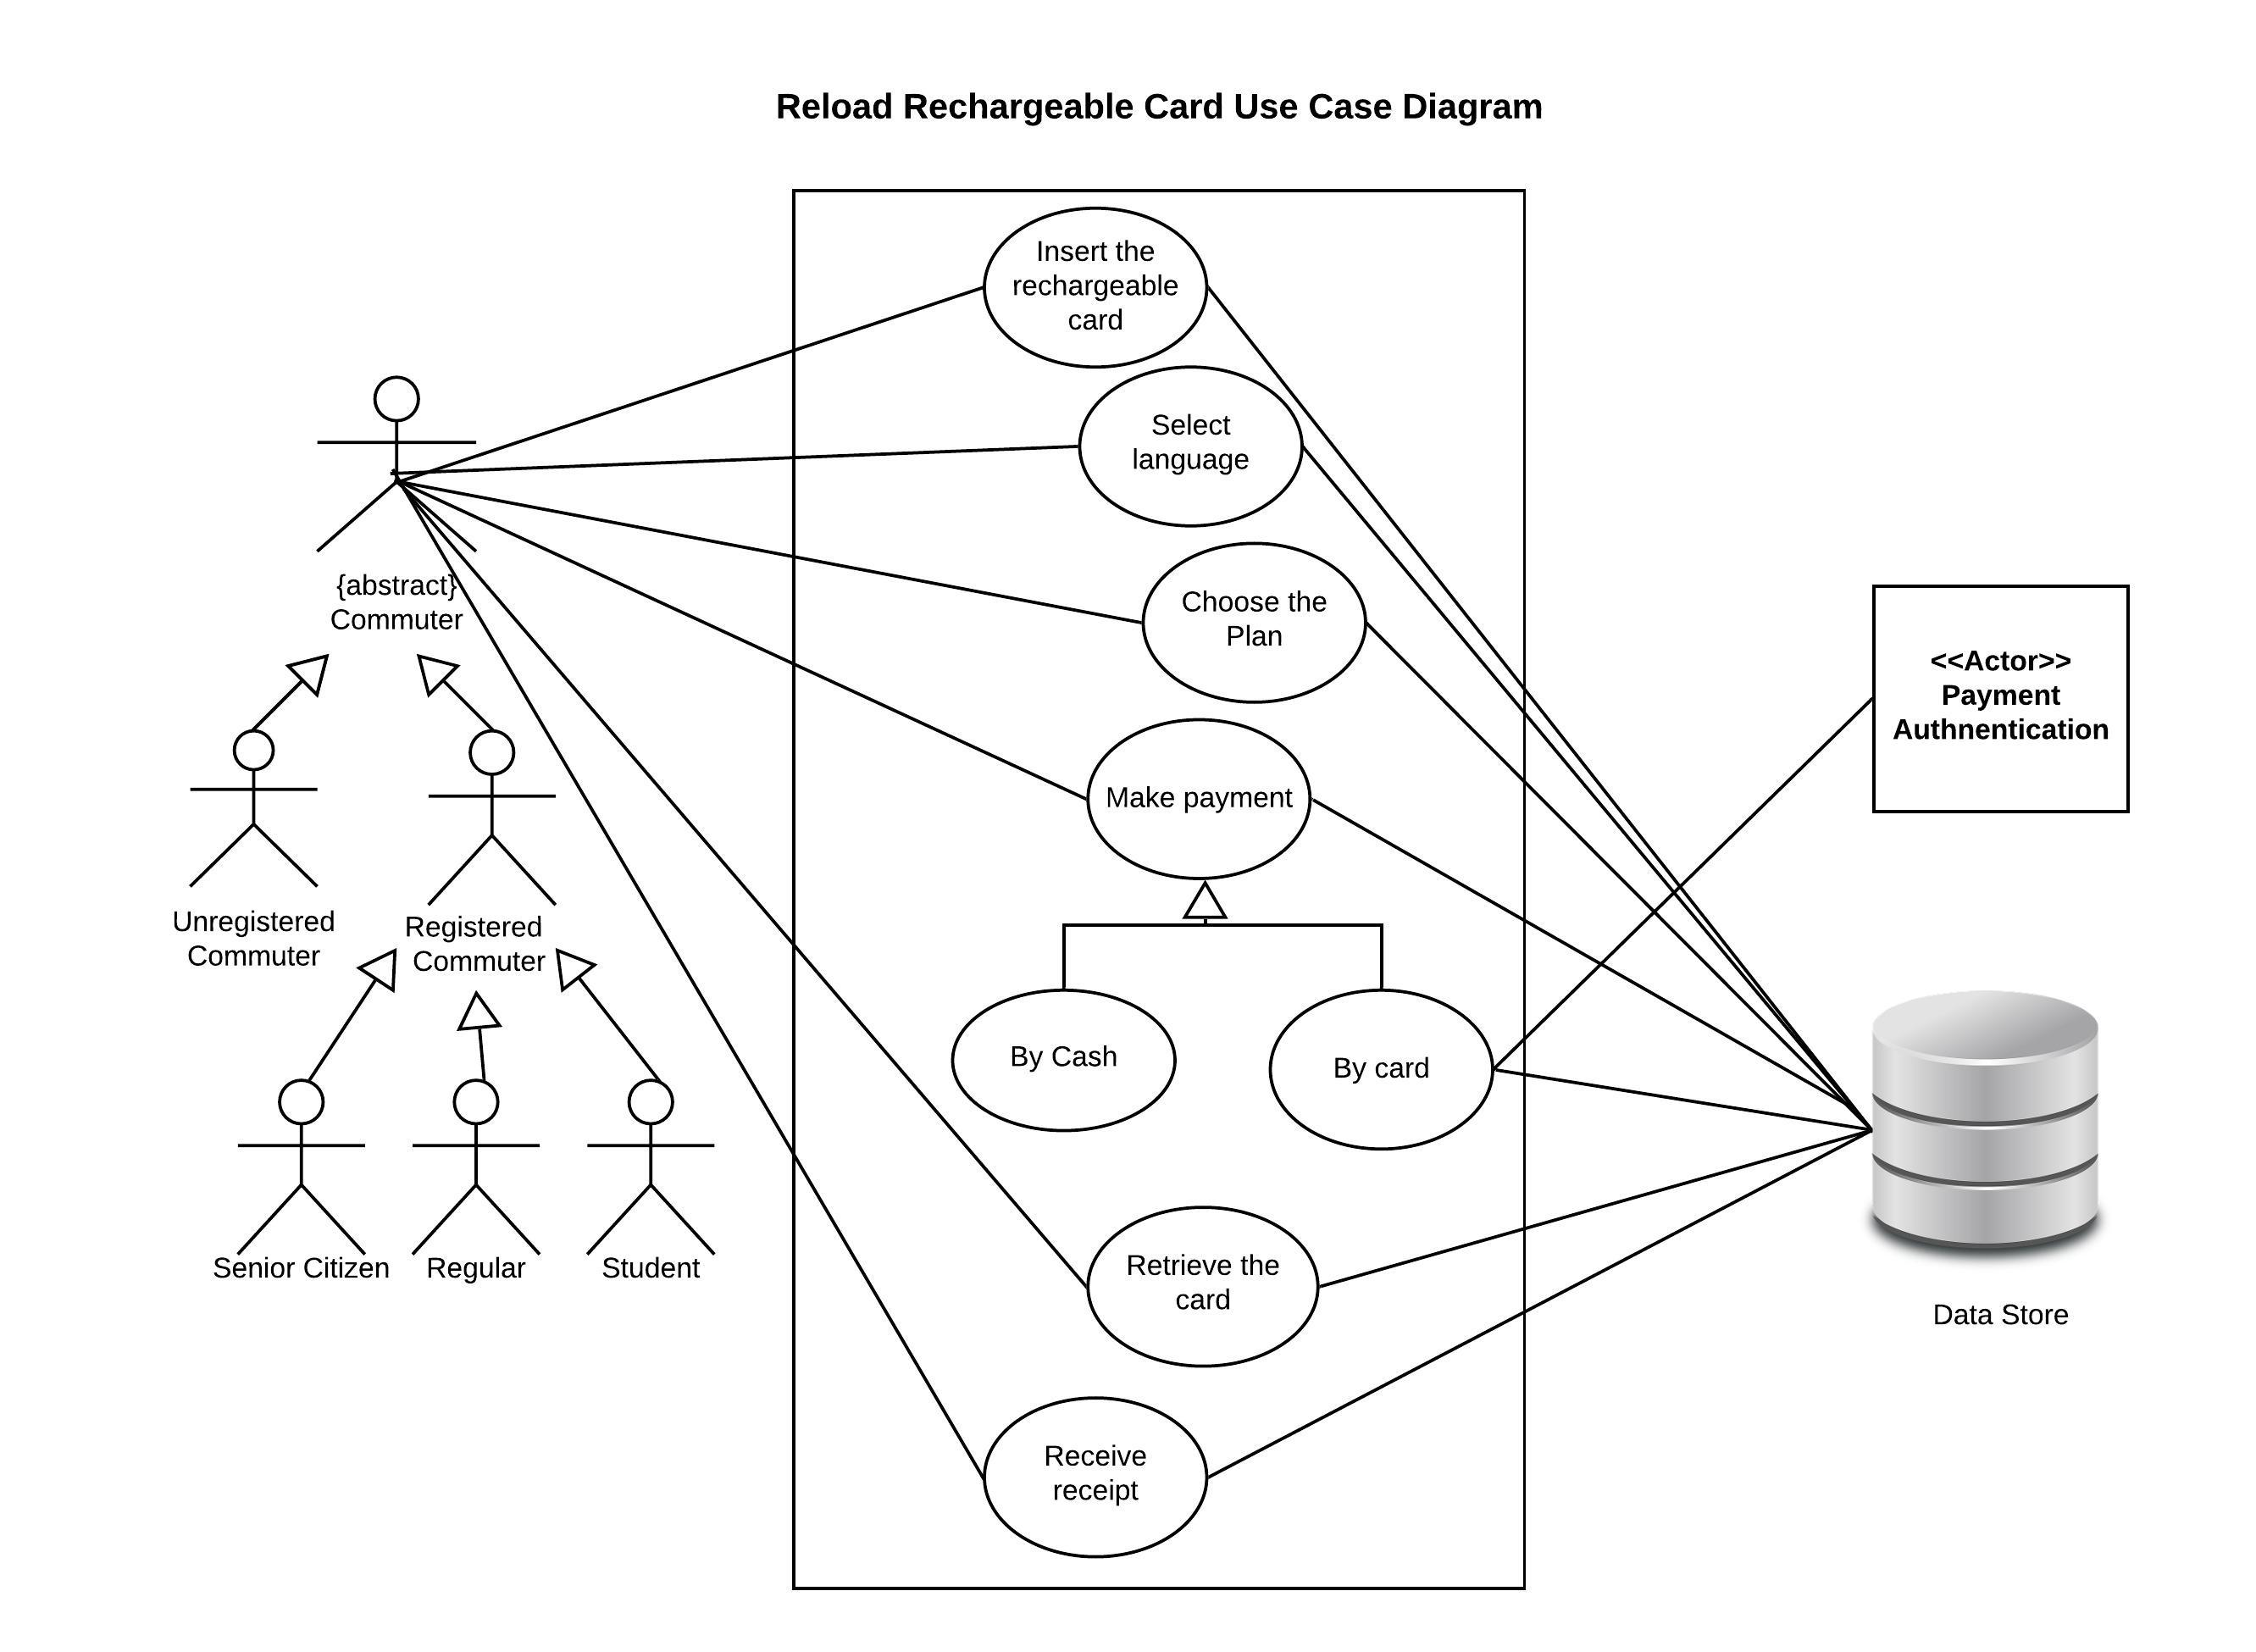
\includegraphics[width=1\textwidth]{Use_Case_Diagrams/ReloadCard.jpeg}}
	\caption{\label{fig:uc_reload_rechargable_card}Use Case: Reload Rechargeable Card}	
\end{figure}

\begin{figure}[!htbp]
	\centering
	\fbox{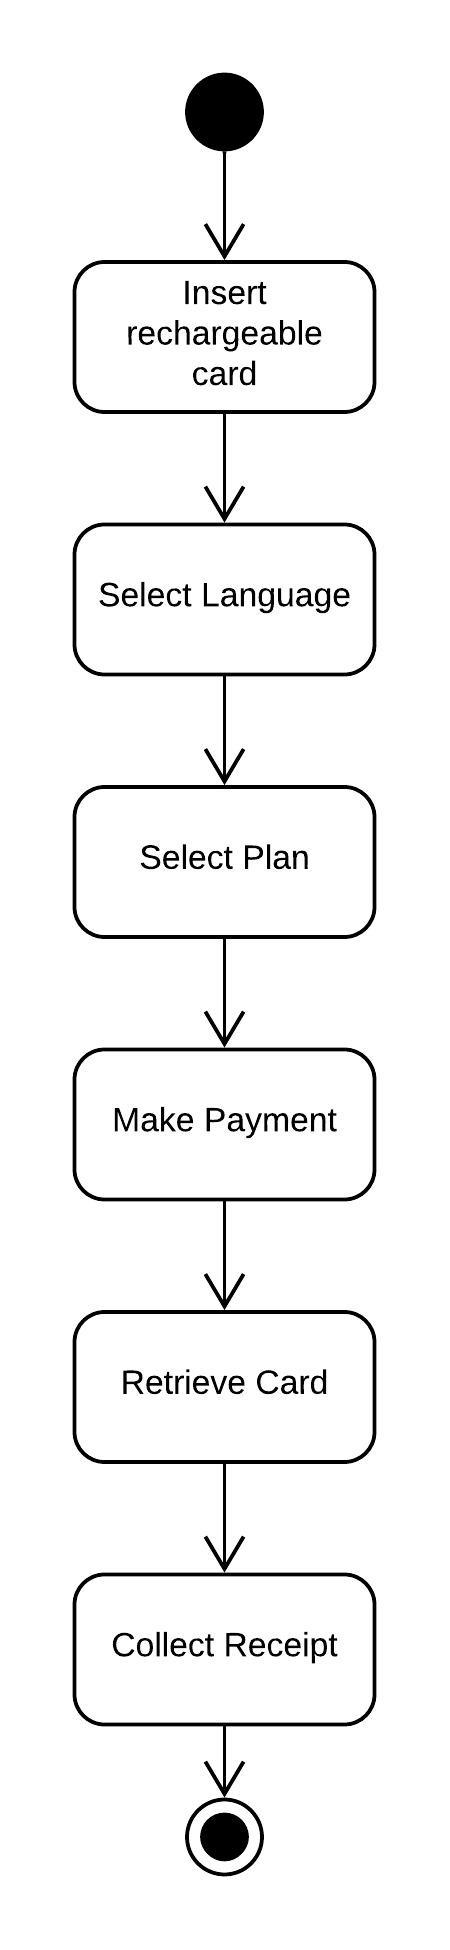
\includegraphics[width=12cm, height=21cm]{Use_Case_Diagrams/ReloadCard_AD.jpeg}}
	\caption{\label{fig:act_reload_rechargable_card}Activity Diagram: Reload Rechargeable Card}	
\end{figure}


\FloatBarrier
\subsection{Use Case: Update Ticket Specification}
Administrator can manage the tickets exiting in the system. He is the primary actor responsible for the Ticket Vending Machine Management. Administrator of the Ticket Vending Machine has the access to create new tickets, modify the existing tickets, view the existing tickets and delete the existing tickets. \\ 

\begin{tabular}{ | c | p{2cm} | p{7cm} |}
	
	\hline
	\textbf{Number} & \multicolumn{2}{c|}{6.1}  \\
	\hline
	\textbf{Name} & \multicolumn{2}{c|}{Create Ticket Specification}  \\
	\hline
	\textbf{Summary} & \multicolumn{2}{c|}{Allows administrator to Create new ticket specifications}  \\
	\hline
	\textbf{Priority} & \multicolumn{2}{c|}{2}  \\
	\hline
	\textbf{Preconditions} & \multicolumn{2}{c|}{The Administrator should have a valid }  \\
			  &  \multicolumn{2	}{c|}{account with valid username and password. The  } \\
			  &  \multicolumn{2	}{c|}{Administrator should be logged into the application} \\
	\hline
	\textbf{Postconditions} & \multicolumn{2}{c|}{Administrator is able to add new ticket plans }  \\
   	 			&  \multicolumn{2}{c|}{to the existing ticket plans. } \\
	\hline
	\textbf{Primary Actor(s)} & \multicolumn{2}{c|}{TVM Administrator}  \\
	\hline
	\textbf{Secondary Actors(s)} & \multicolumn{2}{c|}{TVM and Customer}  \\
	\hline
	\textbf{Trigger} & \multicolumn{2}{c|}{The Administrator has selected to add new}  \\
     	&  \multicolumn{2}{c|}{ ticket specifications to the systems.} \\
	\hline
	\textbf{Main Success Scenarios} & \textbf{Step} & \textbf{Action} \\
	\hline
	& 1 & Admin is given admin access to the system. \\ 
	\hline
	&  2  & Admin creates new ticket plans. \\
	\hline
	&  3  & Ticket details are specified by the admin with new ticket name, expiration date and price. \\
	\hline
	&  4  & The Administrator has added new ticket specifications to the system. \\
	\hline
	
	\textbf{Extensions} & \textbf{Step} & \textbf{Branching Action} \\
	\hline
	&  3a  & Admin does not have the admin access to the system.  \\
	\hline
	&  4a  &  The system gives an error. \\
	\hline
	\textbf{Open Issues} &    & NA \\
	\hline
	
\end{tabular}

\begin{tabular}{ | c | p{2cm} | p{7cm} |}
	
	\hline
	\textbf{Number} & \multicolumn{2}{c|}{6.2}  \\
	\hline
	\textbf{Name} & \multicolumn{2}{c|}{Update Ticket Specification}  \\
	\hline
	\textbf{Summary} & \multicolumn{2}{c|}{Allows administrator to update an}  \\
					&  \multicolumn{2}{c|}{ existing ticket specification. } \\
	\hline
	\textbf{Priority} & \multicolumn{2}{c|}{2}  \\
	\hline
	\textbf{Preconditions} & \multicolumn{2}{c|}{The Administrator should have a valid }  \\
	&  \multicolumn{2	}{c|}{account with valid username and password. The  } \\
	&  \multicolumn{2	}{c|}{Administrator should be logged into the application} \\
	\hline
	\textbf{Postconditions} & \multicolumn{2}{c|}{Administrator is able to edit ticket plans }  \\
							&  \multicolumn{2}{c|}{to the existing ticket plans. } \\
	\hline
	\textbf{Primary Actor(s)} & \multicolumn{2}{c|}{TVM Administrator}  \\
	\hline
	\textbf{Secondary Actors(s)} & \multicolumn{2}{c|}{TVM and Customer}  \\
	\hline
	\textbf{Trigger} & \multicolumn{2}{c|}{The Administrator has selected to update}  \\
	&  \multicolumn{2}{c|}{ ticket specifications on the systems.} \\
	\hline
	\textbf{Main Success Scenarios} & \textbf{Step} & \textbf{Action} \\
	\hline
	& 1 & Admin selects the tickets to be modified. \\ 
	\hline
	&  2  & Admin change the ticket specification. \\
	\hline
	&  3  & Admin saves the new ticket specifications. \\
	\hline
	&  4  & Admin updates the system with updated ticket plans. \\
	\hline
	
	\textbf{Extensions} & \textbf{Step} & \textbf{Branching Action} \\
	\hline
	&  3a  & Admin does not have the admin access to the system.  \\
	\hline
	&  4a  &  The system gives an error. \\
	\hline
	\textbf{Open Issues} &    & NA \\
	\hline
	
\end{tabular}

\begin{tabular}{ | c | p{2cm} | p{7cm} |}
	
	\hline
	\textbf{Number} & \multicolumn{2}{c|}{6.3}  \\
	\hline
	\textbf{Name} & \multicolumn{2}{c|}{Delete Ticket Specification}  \\
	\hline
	\textbf{Summary} & \multicolumn{2}{c|}{Allows administrator to delete }  \\
					& \multicolumn{2}{c|}{existing ticket specifications}  \\
	\hline
	\textbf{Priority} & \multicolumn{2}{c|}{2}  \\
	\hline
	\textbf{Preconditions} & \multicolumn{2}{c|}{The Administrator should have a valid }  \\
	&  \multicolumn{2	}{c|}{account with valid username and password. The  } \\
	&  \multicolumn{2	}{c|}{Administrator should be logged into the application} \\
	\hline
	\textbf{Postconditions} & \multicolumn{2}{c|}{Administrator is able to delete ticket plan }  \\
	&  \multicolumn{2}{c|}{from system. } \\
	\hline
	\textbf{Primary Actor(s)} & \multicolumn{2}{c|}{TVM Administrator}  \\
	\hline
	\textbf{Secondary Actors(s)} & \multicolumn{2}{c|}{TVM and Customer}  \\
	\hline
	\textbf{Trigger} & \multicolumn{2}{c|}{The Administrator has selected to delete}  \\
	&  \multicolumn{2}{c|}{ ticket specifications on the systems.} \\
	\hline
	\textbf{Main Success Scenarios} & \textbf{Step} & \textbf{Action} \\
	\hline
	& 1 & Admin selects the tickets to be changed. \\ 
	\hline
	&  2  & Admin deletes the selected ticket specification. \\
	\hline
	&  3  & The system is updated after deleting. \\
	\hline
	&  4  & Application updates the list of new tickets available. \\
	\hline
	
	\textbf{Extensions} & \textbf{Step} & \textbf{Branching Action} \\
	\hline
	&  3a  & Admin does not have the admin access to the system.  \\
	\hline
	&  4a  &  The system gives an error. \\
	\hline
	\textbf{Open Issues} &    & NA \\
	\hline
	
\end{tabular}



\begin{figure}[!htbp]
	\centering
	\fbox{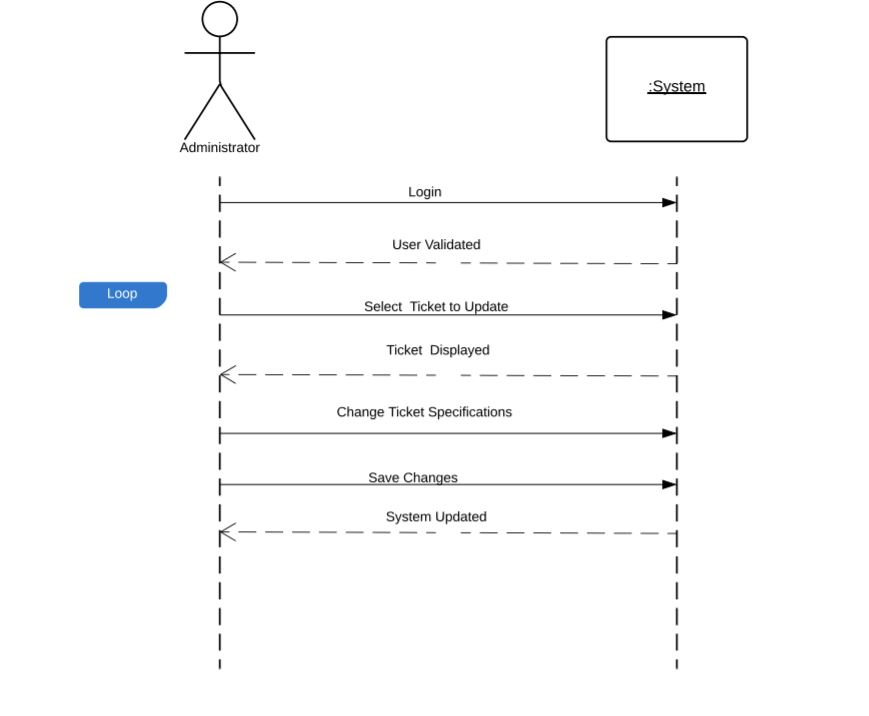
\includegraphics[width=1\textwidth]{Use_Case_Diagrams/admin_system_seq.JPG}}
	\caption{\label{fig:seq_admin_system} Sequence Diagram: Admin Sytem}	
\end{figure}


\FloatBarrier
\subsection{Use Case: Customer Registration}
Commuter(New User) use Ticket Vending Machine to register himself/herself with the STM. Commuter is the primary actor that initiate the use case by choosing the register option. Secondary actor includes Data Store that supports and responds to the requests. The result for a normal use case scenario is that the customer got registered with the STM. Figure~\ref{fig:uc_customer_registration} and~\ref{fig:act_customer_registration} explain this use case. \\ 


\begin{tabular}{ | c | p{2cm} | p{7cm} |}
	
	\hline
	\textbf{Number} & \multicolumn{2}{c|}{7}  \\
	\hline
	\textbf{Name} & \multicolumn{2}{c|}{Customer Registration}  \\
	\hline
	\textbf{Summary} & \multicolumn{2}{c|}{Customer register with his personal}\\
					  & \multicolumn{2}{c|}{information to get the card}  \\
	\hline
	\textbf{Priority} & \multicolumn{2}{c|}{2}  \\
	\hline
	\textbf{Preconditions} & \multicolumn{2}{c|}{N/A}  \\
	\hline
	\textbf{Postconditions} & \multicolumn{2}{c|}{User is registered}  \\
	\hline
	\textbf{Primary Actor(s)} & \multicolumn{2}{c|}{TVM Customer}  \\
	\hline
	\textbf{Secondary Actors(s)} & \multicolumn{2}{c|}{Data Store}  \\
	\hline
	\textbf{Trigger} & \multicolumn{2}{c|}{User has chosen to register himself for the STM} \\
	\hline
	\textbf{Main Success Scenarios} & \textbf{Step} & \textbf{Action} \\
	\hline
	& 1 & User selects the register option \\ 
	\hline
	&  2  & System asks for his personal identification information \\
	\hline
	&  3  & User fills all the information and submit it \\
	\hline
	&  4  & System asks for the username and password \\
	\hline
	&  5  & User creates a username and password \\
	\hline
	&  6  & System checks for the validity of the user \\
	\hline
	&  7  & System registers the user and shows a registered user message \\
	\hline

	\textbf{Extensions} & \textbf{Step} & \textbf{Branching Action} \\
	\hline
	\textbf{Open Issues} &    & NA \\
	\hline

\end{tabular}


\begin{figure}[!htbp]
	\fbox{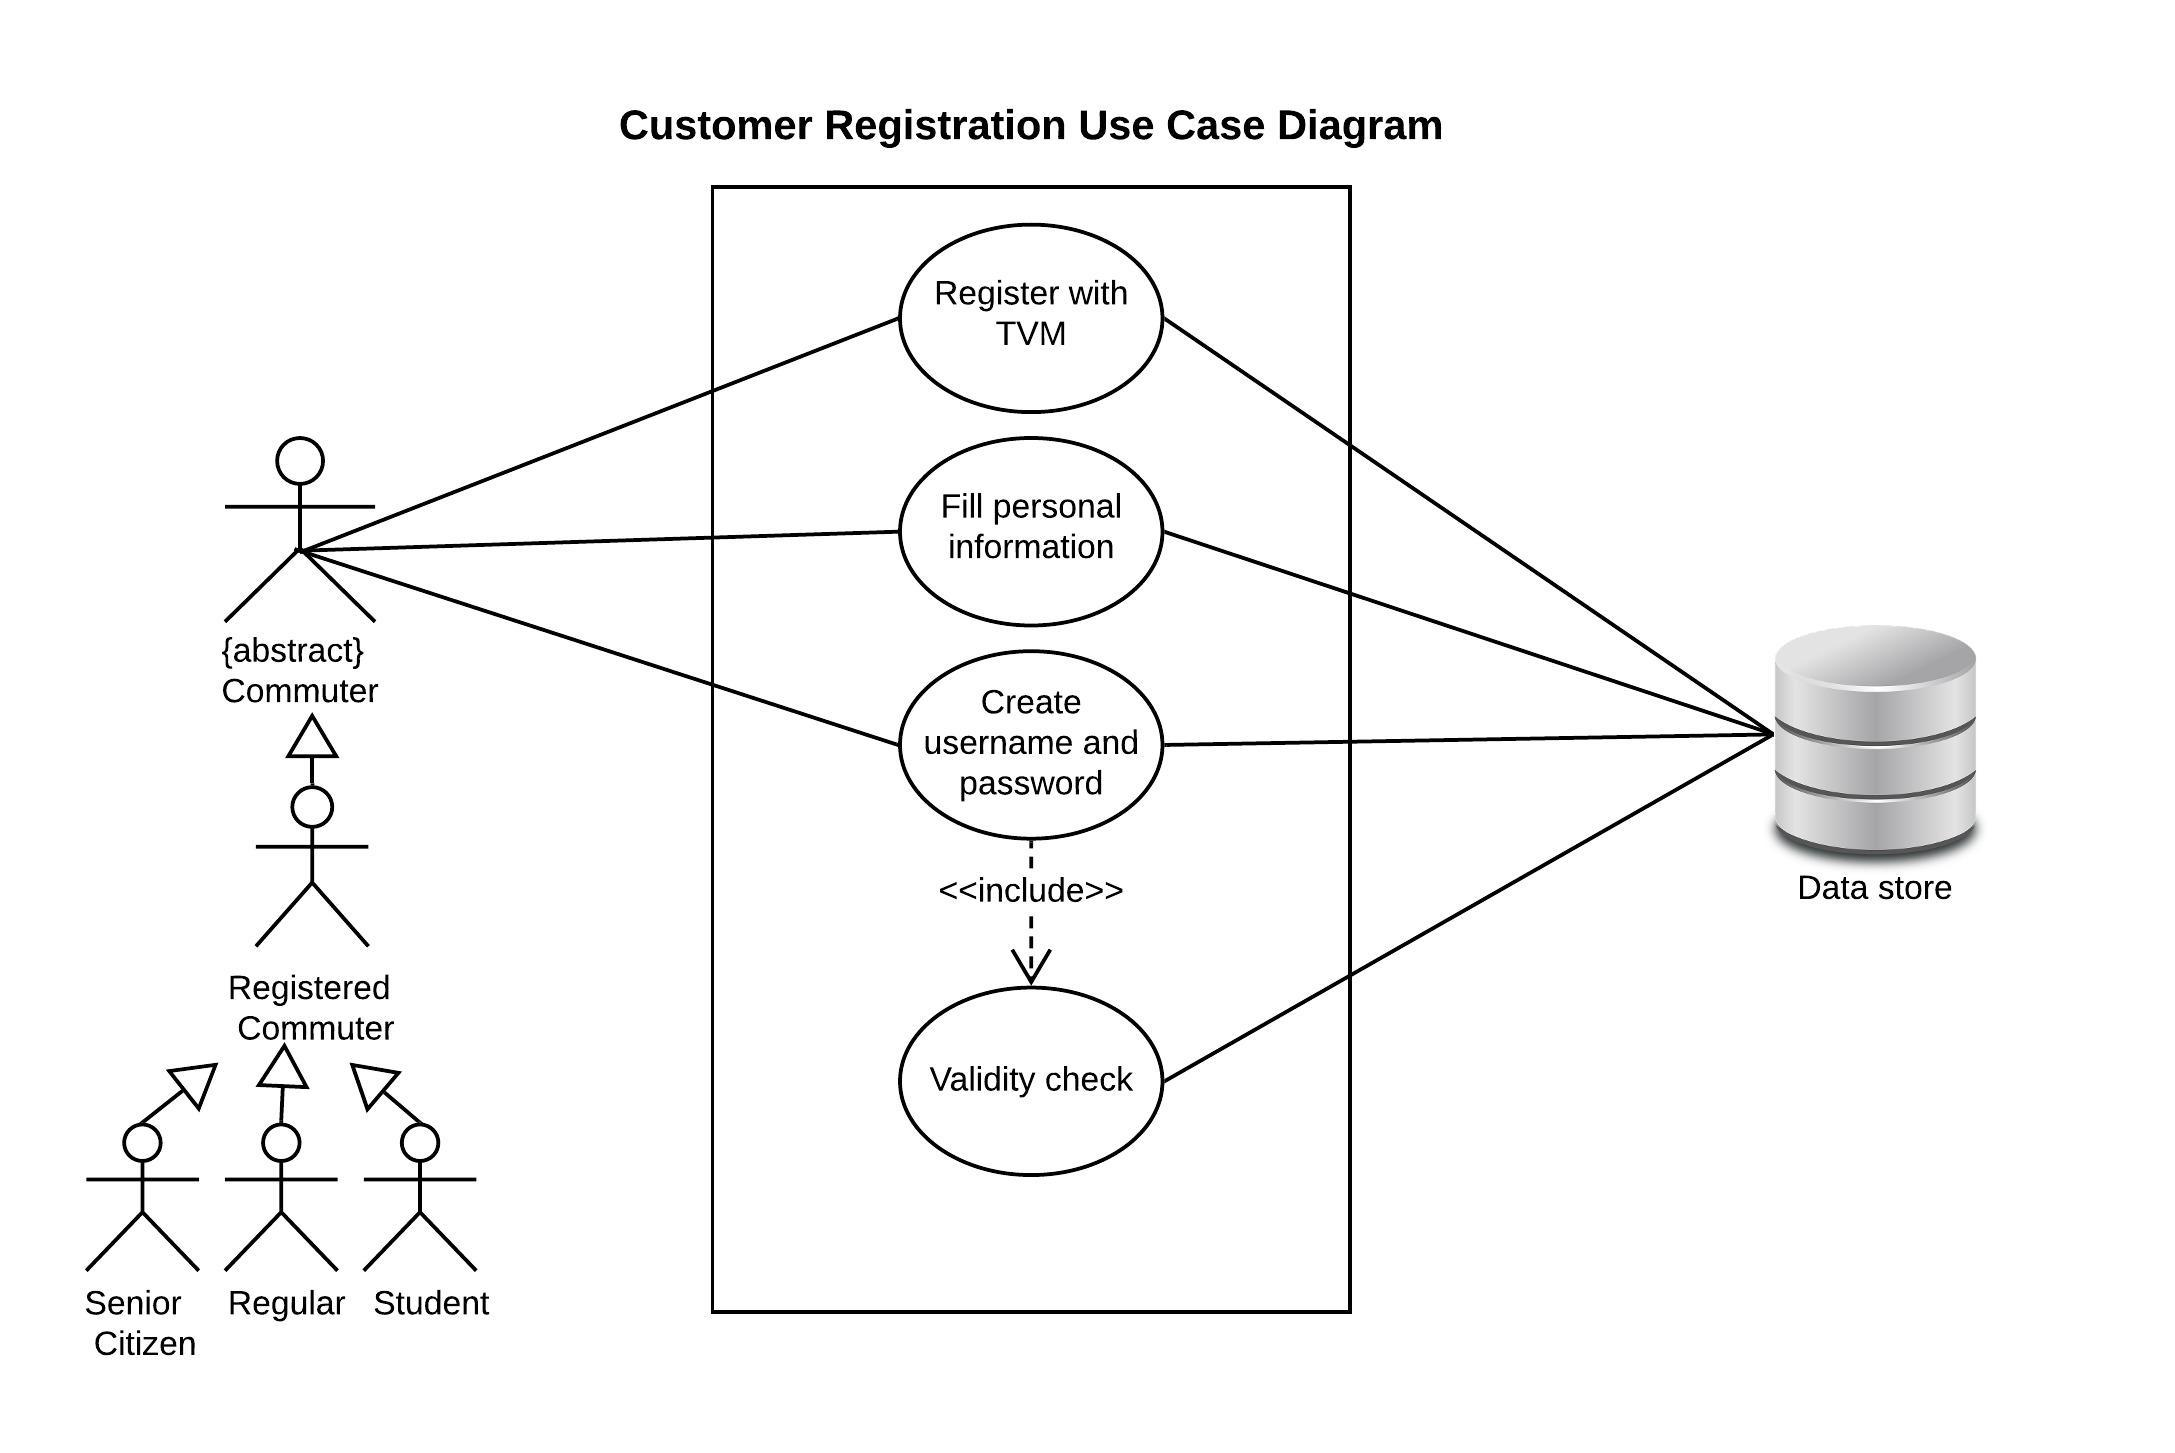
\includegraphics[width=18cm, height=16cm]{Use_Case_Diagrams/CustomerRegistration.jpeg}}
	\caption{\label{fig:uc_customer_registration}Use Case: Customer Registration}	
\end{figure}


\begin{figure}[!htbp]
	\centering
	\fbox{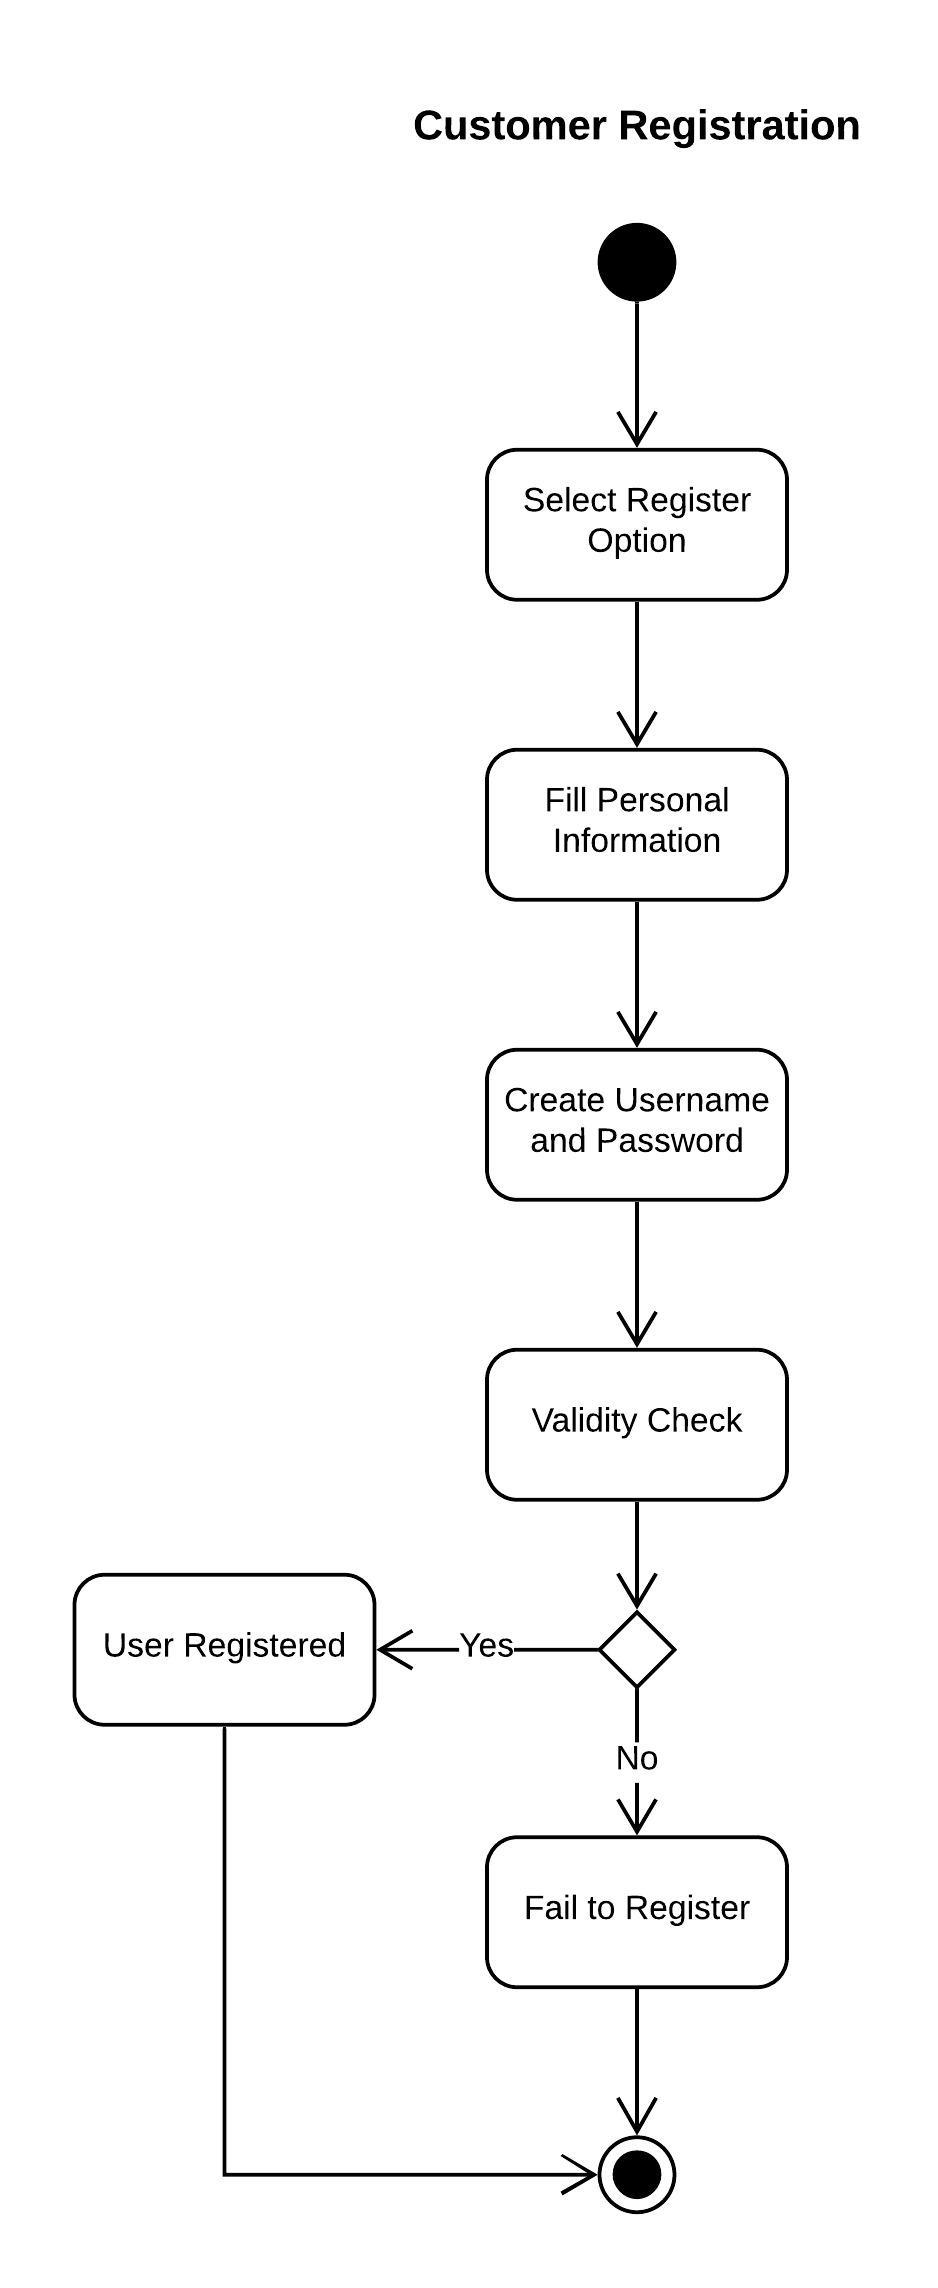
\includegraphics[width=12cm,height=20cm]{Use_Case_Diagrams/Customer_Registration_AD.jpeg}}
	\caption{\label{fig:act_customer_registration}Activity Diagram: Customer Registration}	
\end{figure}



\FloatBarrier
\subsection{Use Case: False Login}

\begin{tabular}{ | c | p{2cm} | p{7cm} |}
	
	\hline
	\textbf{Number} & \multicolumn{2}{c|}{7}  \\
	\hline
	\textbf{Name} & \multicolumn{2}{c|}{False Login}  \\
	\hline
	\textbf{Summary} & \multicolumn{2}{c|}{Hacker try to login into someone else account.}  \\
	\hline
	\textbf{Priority} & \multicolumn{2}{c|}{1}  \\
	\hline
	\textbf{Preconditions} & \multicolumn{2}{c|}{N/A}  \\
	\hline
	\textbf{Postconditions} & \multicolumn{2}{c|}{Login should fail with appropriate error message.}  \\
	\hline
	\textbf{Primary Actor(s)} & \multicolumn{2}{c|}{Hacker / TVM.}  \\
	\hline
	\textbf{Secondary Actors(s)} & \multicolumn{2}{c|}{Data Store}  \\
	\hline
	\textbf{Trigger} & \multicolumn{2}{c|}{User account locked after 5 unsuccessful login attempts.} \\
	\hline
	\textbf{Main Success Scenarios} & \textbf{Step} & \textbf{Action} \\
	\hline
	& 1 & Hacker try to login into system. \\ 
	\hline
	&  2  & Hacker enters username and password. \\
	\hline
	&  3  & System will validate user details from database system. \\
	\hline
	&  4  & System decline unauthorized access. System should display appropriate error message. \\
	\hline
	&  5  & System should display appropriate error message. \\
	\hline
	&  6  & Hacker keeps on entering invalid credentials to try to login into someone account. \\
	\hline
	&  7  & System will lock user account after 5 unsuccessful login attempts. \\
	\hline
	& 8 & System should display account locked error message to user. \\
	\hline
	
	\textbf{Extensions} & \textbf{Step} & \textbf{Branching Action} \\
	\hline
	\textbf{Open Issues} &    & NA \\
	\hline
	
\end{tabular}


\FloatBarrier
\subsection{Use Case: Password Reset}
\subsubsection{Use Case Diagram}
The password reset use case diagram explains how a customer will be able to reset the password of his/her account. The password reset will include another use case called authenticate. This can be either by security questions or by email.

\begin{figure}[!htbp]
	\fbox{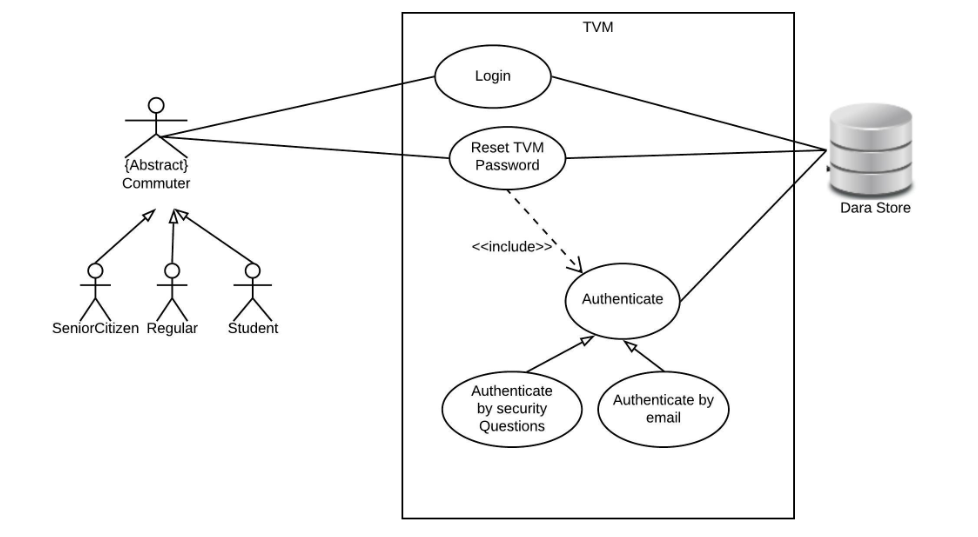
\includegraphics[width=1\textwidth]{Use_Case_Diagrams/PasswordReset_UCD.jpeg}}
	\caption{\label{fig: uc_password_reset } Use Case Diagram: Password Reset}	
\end{figure}


\subsubsection{Activity Diagram}
The activity diagram is for the Password reset. The sequential steps are as shown, and if the password change authentication fails, the process will be terminated.

\begin{figure}[!htbp]
	\fbox{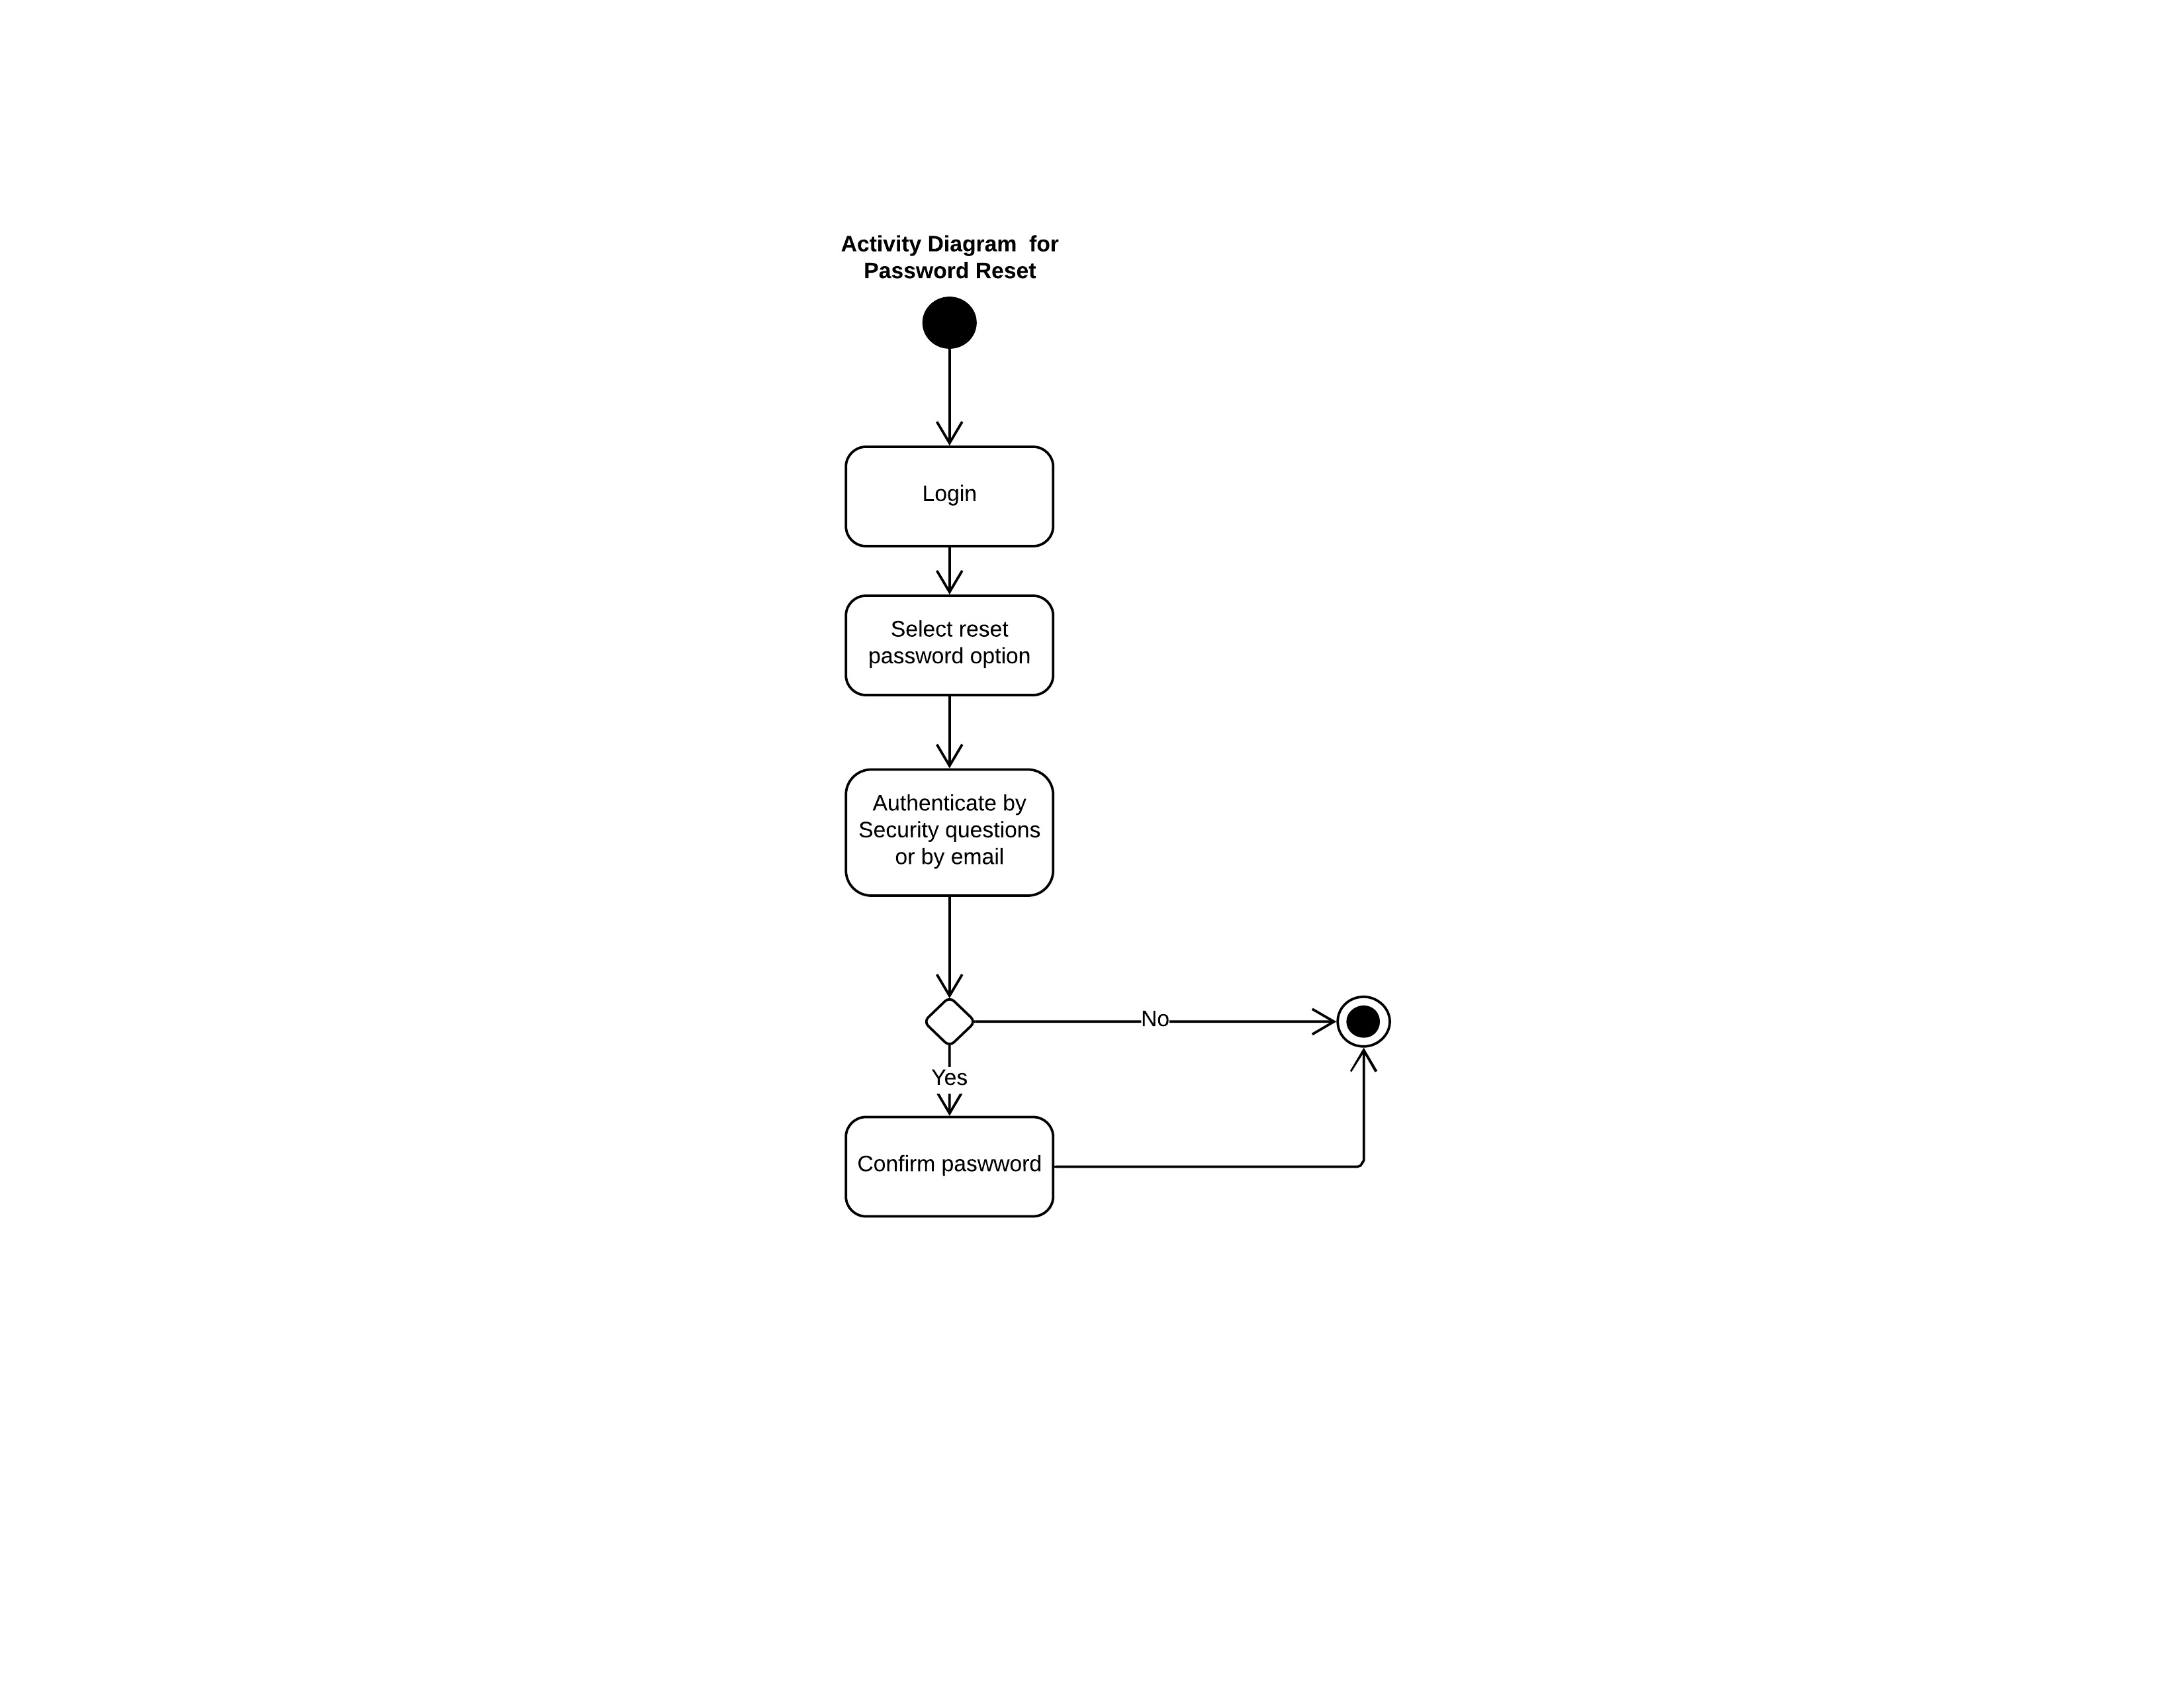
\includegraphics[width=1\textwidth]{Use_Case_Diagrams/PasswordReset_AD.jpeg}}
	\caption{\label{fig: act_password_reset } Activity Diagram: Password Reset}	
\end{figure}


\FloatBarrier
\subsection{Use Case: Payment Fraud}
The Payment Fraud use case diagram shows how the payment authentication use case can be threatened by the negative use case called Flood system and Steal card information. The name of the use cases explains the activity of negative use cases. \\

\begin{figure}[!htbp]
	\fbox{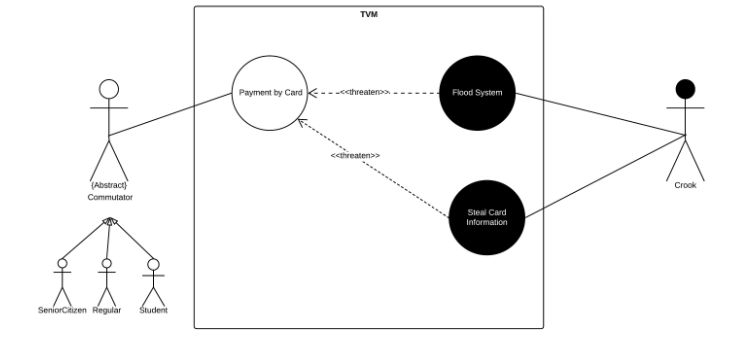
\includegraphics[width=1\textwidth]{Use_Case_Diagrams/PaymentFraud_UCD.jpeg}}
	\caption{\label{fig: uc_payment_fraud } Use Case Diagram: Payment Fraud}	
\end{figure}

%=================================================================
%
%					APPENDIX PAGE
%
%==================================================================

\printbibliography[heading=subbibliography,title=References]

\printglossaries

\appendix
\addcontentsline{toc}{section}{Appendices}
\renewcommand{\thesection}{\Alph{section}}
\section{Appendix}
\subsection{Interviews}
Users are Interviewed and the results are accessable at: \href{https://github.com/m3hrn4z/SRS}{https://github.com/m3hrn4z/SRS}




\end{document}

